\subsection{Pré-traitement}\label{subsec:pre-traitement}
On regarde le nombre de \texttt{\#}, \texttt{@} et lien par tweet selon le type de tweet scientifique (\autoref{fig:hashtag_count}).

\begin{figure}[H]
    \centering
    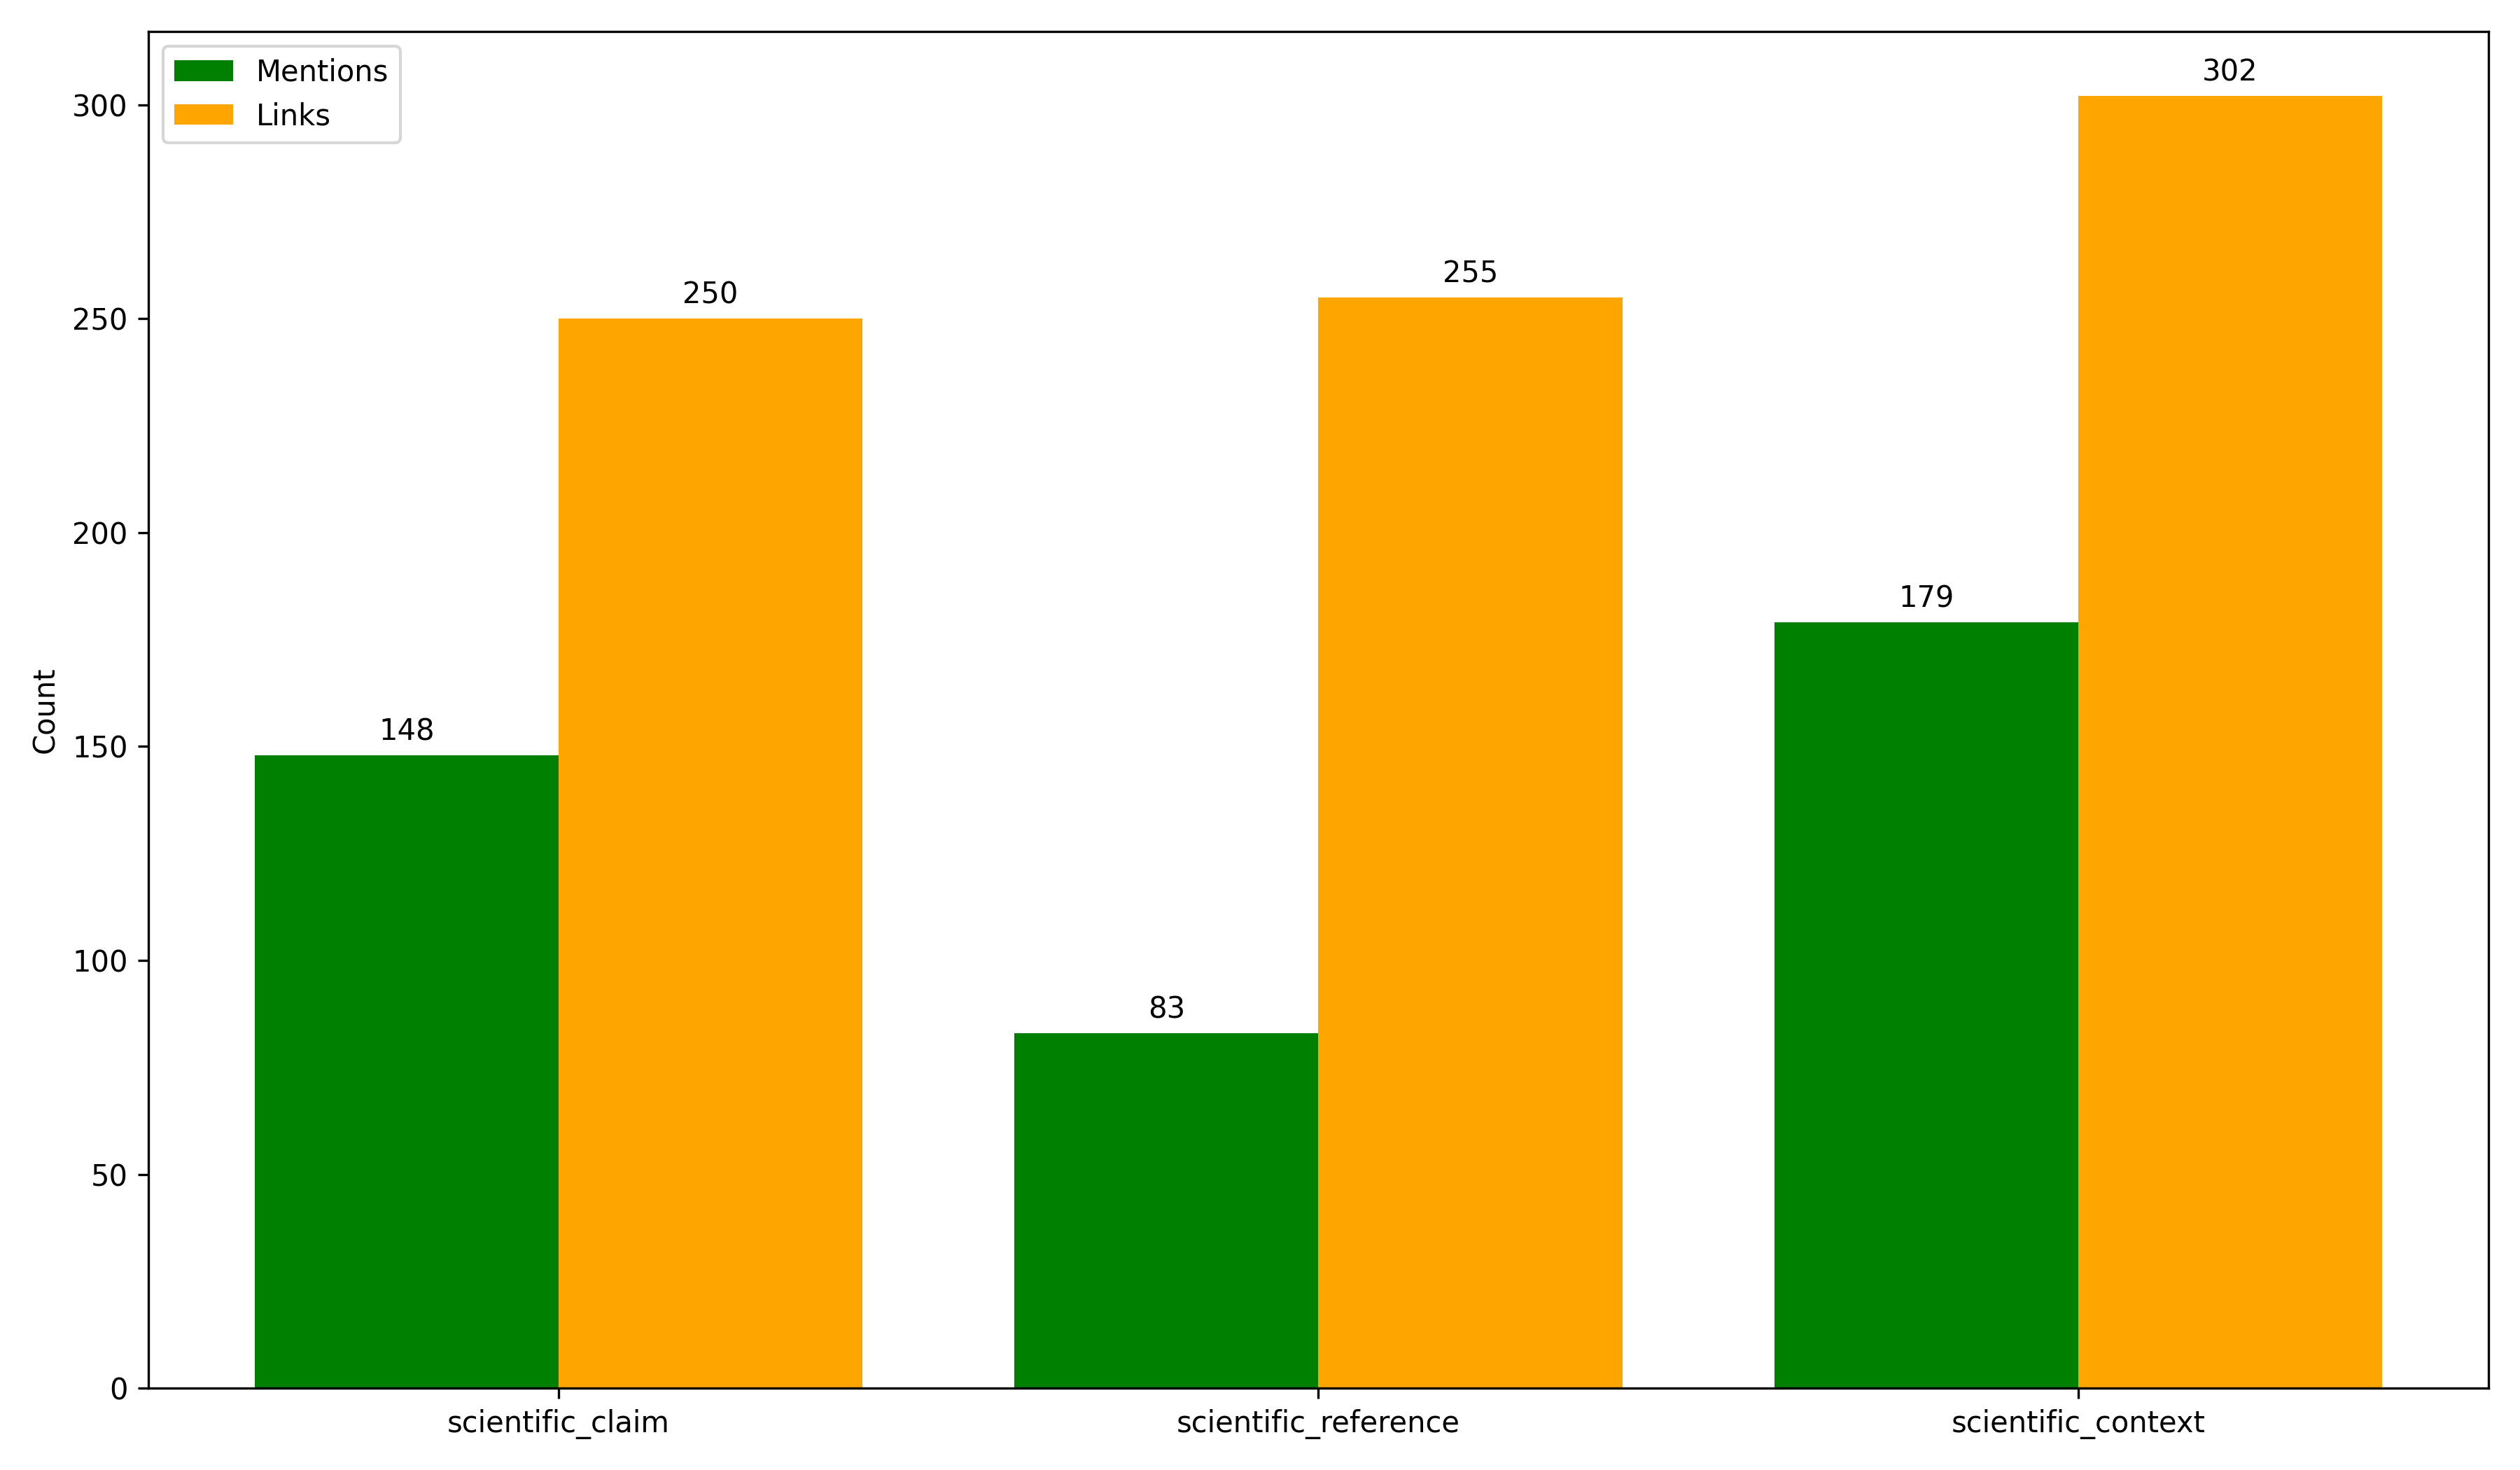
\includegraphics[width=1\textwidth]{images/hashtag_links_mentions_count_outliers}
    \caption{Nombre de hashtags par tweet selon le type de tweet scientifique.}
    \label{fig:hashtag_count}
\end{figure}

Après avoir réalisé des tests d'indépendance de student sur chaque variable, les \textit{p-values} ne descendent pas en dessous de 0.18 donc on ne remarque pas de différence significative entre les tweets scientifiques et non scientifiques.
On peut ainsi conclure que ces variables ne sont pas pertinentes pour la classification des tweets scientifiques, on les retirera de notre dataset.
Malgrès tout, les \texttt{\#} permettent une meilleur accuracy overall, on l'a donc gardé.

\subsection{Modélisation}\label{subsec:modelisation}
Dans cette section, nous comparons les performances des modèles sur trois tâches de classification hiérarchiques successives.
Par la suite, nous présentons les résultats de classification obtenus pour chaque tâche ainsi qu’une comparaison des performances des approches utilisées.

\noindent Pour chacunes des étapes, nous allons comparer différents modèles entre eux pour sélectionner le meilleur modèle.
Par meilleur modèle, on entend la meilleure précision et le plus petit écart-type.
Chaque modèle est testé par cross-validation sur 10 itérations.

\subsection{Modèle 1: Scientifique versus Non Scientifique}\label{subsec:modele-1:-sci-vs-non-sci}
Dans cette tâche, nous avons comparé plusieurs modèles de classification afin de distinguer les tweets scientifiques des non-scientifiques.
L’objectif était d’évaluer les performances de différentes approches d’apprentissage supervisé appliquées à un problème de classification binaire.

\subsubsection{Préparation des données}
Nous avons supprimé les mentions (@), les caractères spéciaux et converti l’ensemble des textes en minuscules, pour standardiser l’entrée pour éviter que des variations superficielles n’influencent la classification.
Une liste de stopwords a été utilisée, combinant celle de NLTK et des termes propres à Twitter ("http", "https", "rt", "co", "amp", "via") qui sont fréquents mais peu informatifs pour déterminer la nature scientifique du contenu.
Pour la vectorisation, nous avons utilisé la méthode TF-IDF avec des n-grammes de taille 1 à 2, un choix raisonnable pour capturer à la fois des mots individuels et des associations fréquentes, tout en limitant la complexité.

Étant donné le fort déséquilibre des classes (la classe SCI représentant moins de 10 \%), la technique SMOTE a été utilisée pour équilibrer la distribution entre classes SCI et NON-SCI.

\subsubsection{Analyse comparative des performances des différents modèles}
Plusieurs modèles de classification ont été testés (\autoref{tab:model_comparison_sci_nsci}).
Chacun a été optimisé à l’aide d’une recherche par grille (GridSearchCV) et évalué à l’aide d’une validation croisée à 10 plis (KFold), afin d’identifier les meilleures combinaisons d’hyperparamètres.

\begin{table}[H]
    \centering
    \caption{Performances des modèles - Tâche 1}
    \begin{tabular}{lcccc}
        \toprule
        Modèle & Accuracy (\autoref{fig:model_comparison_sci_nsci}) & Précision (\autoref{fig:confusion_1.json-logistic-regression_sci_confusion_matrix}) & Rappel (\autoref{fig:confusion_1.json-logistic-regression_sci_confusion_matrix}) & F1-score \\
        \midrule
        Logistic Regression & 0.9327 & 0.93 & 0.93 & 0.93 \\
        Naive Bayes & 0.9092 & 0.91 & 0.90 & 0.90 \\
        k-NN & 0.8092 & 0.83 & 0.80 & 0.80 \\
        Random Forest & 0.8680 & 0.86 & 0.84 & 0.83 \\
        SVM (linéaire) & 0.9412 & 0.94 & 0.94 & 0.94 \\
        \bottomrule
    \end{tabular}\label{tab:model_comparison_sci_nsci}
\end{table}

\noindent Le modèle SVM semble être le plus performant pour cette tâche, affichant les meilleurs scores en précision, rappel et F1-score, ainsi qu’une accuracy élevée accompagnée mais un plus grand écart-type que la régression logistique \autoref{fig:model_comparison_sci_nsci}.
C'est pour cette raison de stabilité que l'on préfèrera la régression logistique car elle présente une baisse de performance négligeable comparé à la stabilité du modèle.

\begin{figure}[H]
    \centering
    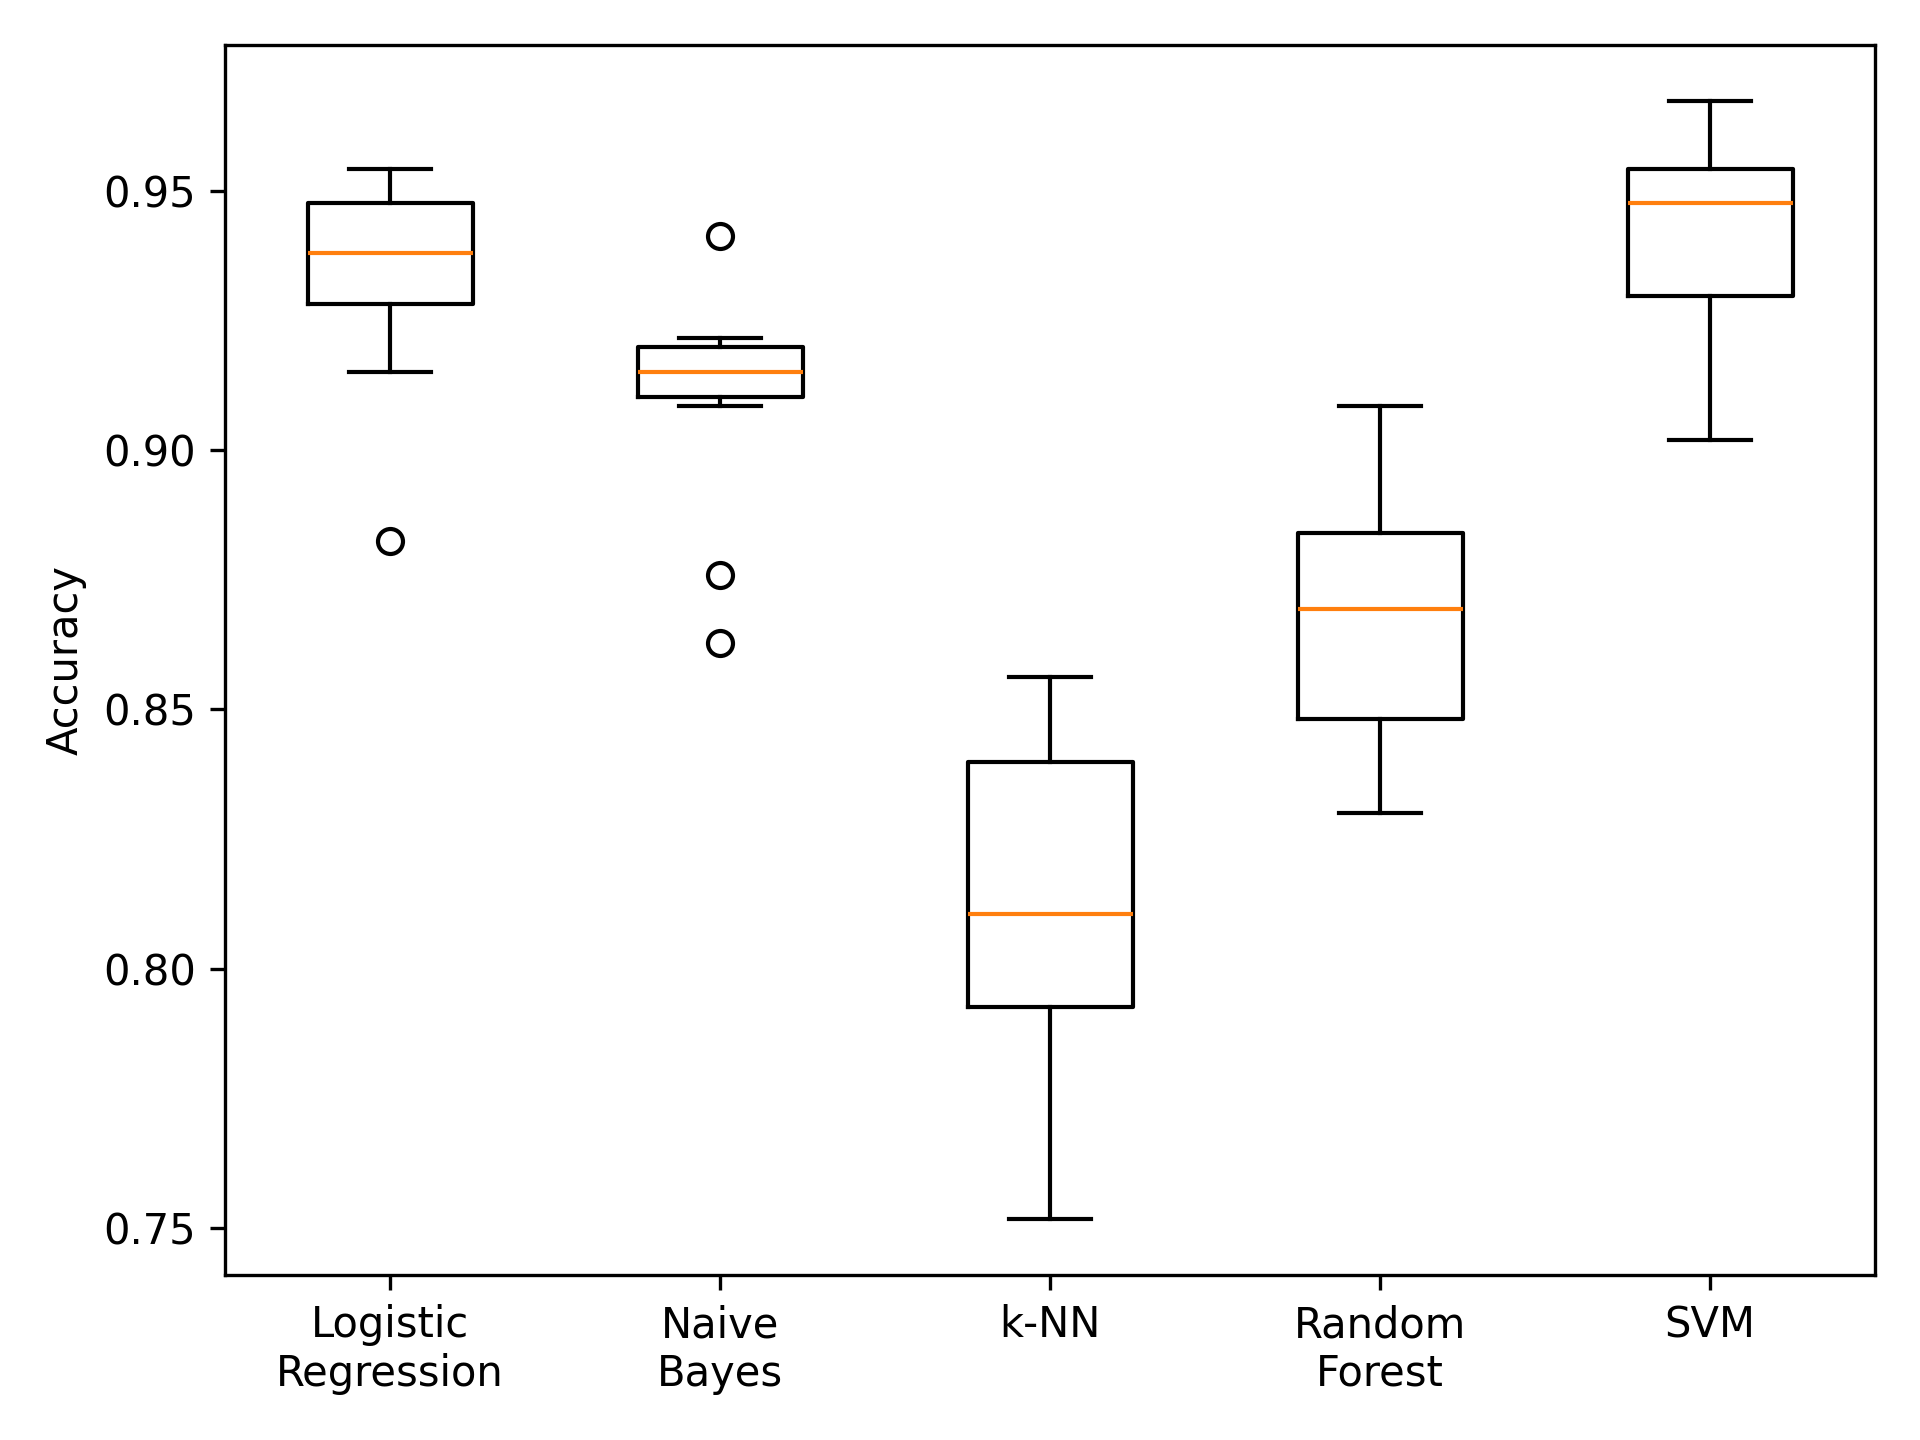
\includegraphics[width=0.75\textwidth]{images/model_comparison_1}
    \caption{Comparaison des modèles pour la classification des tweets scientifiques et non scientifiques.}
    \label{fig:model_comparison_sci_nsci}
\end{figure}

\begin{figure}[H]
    \centering
    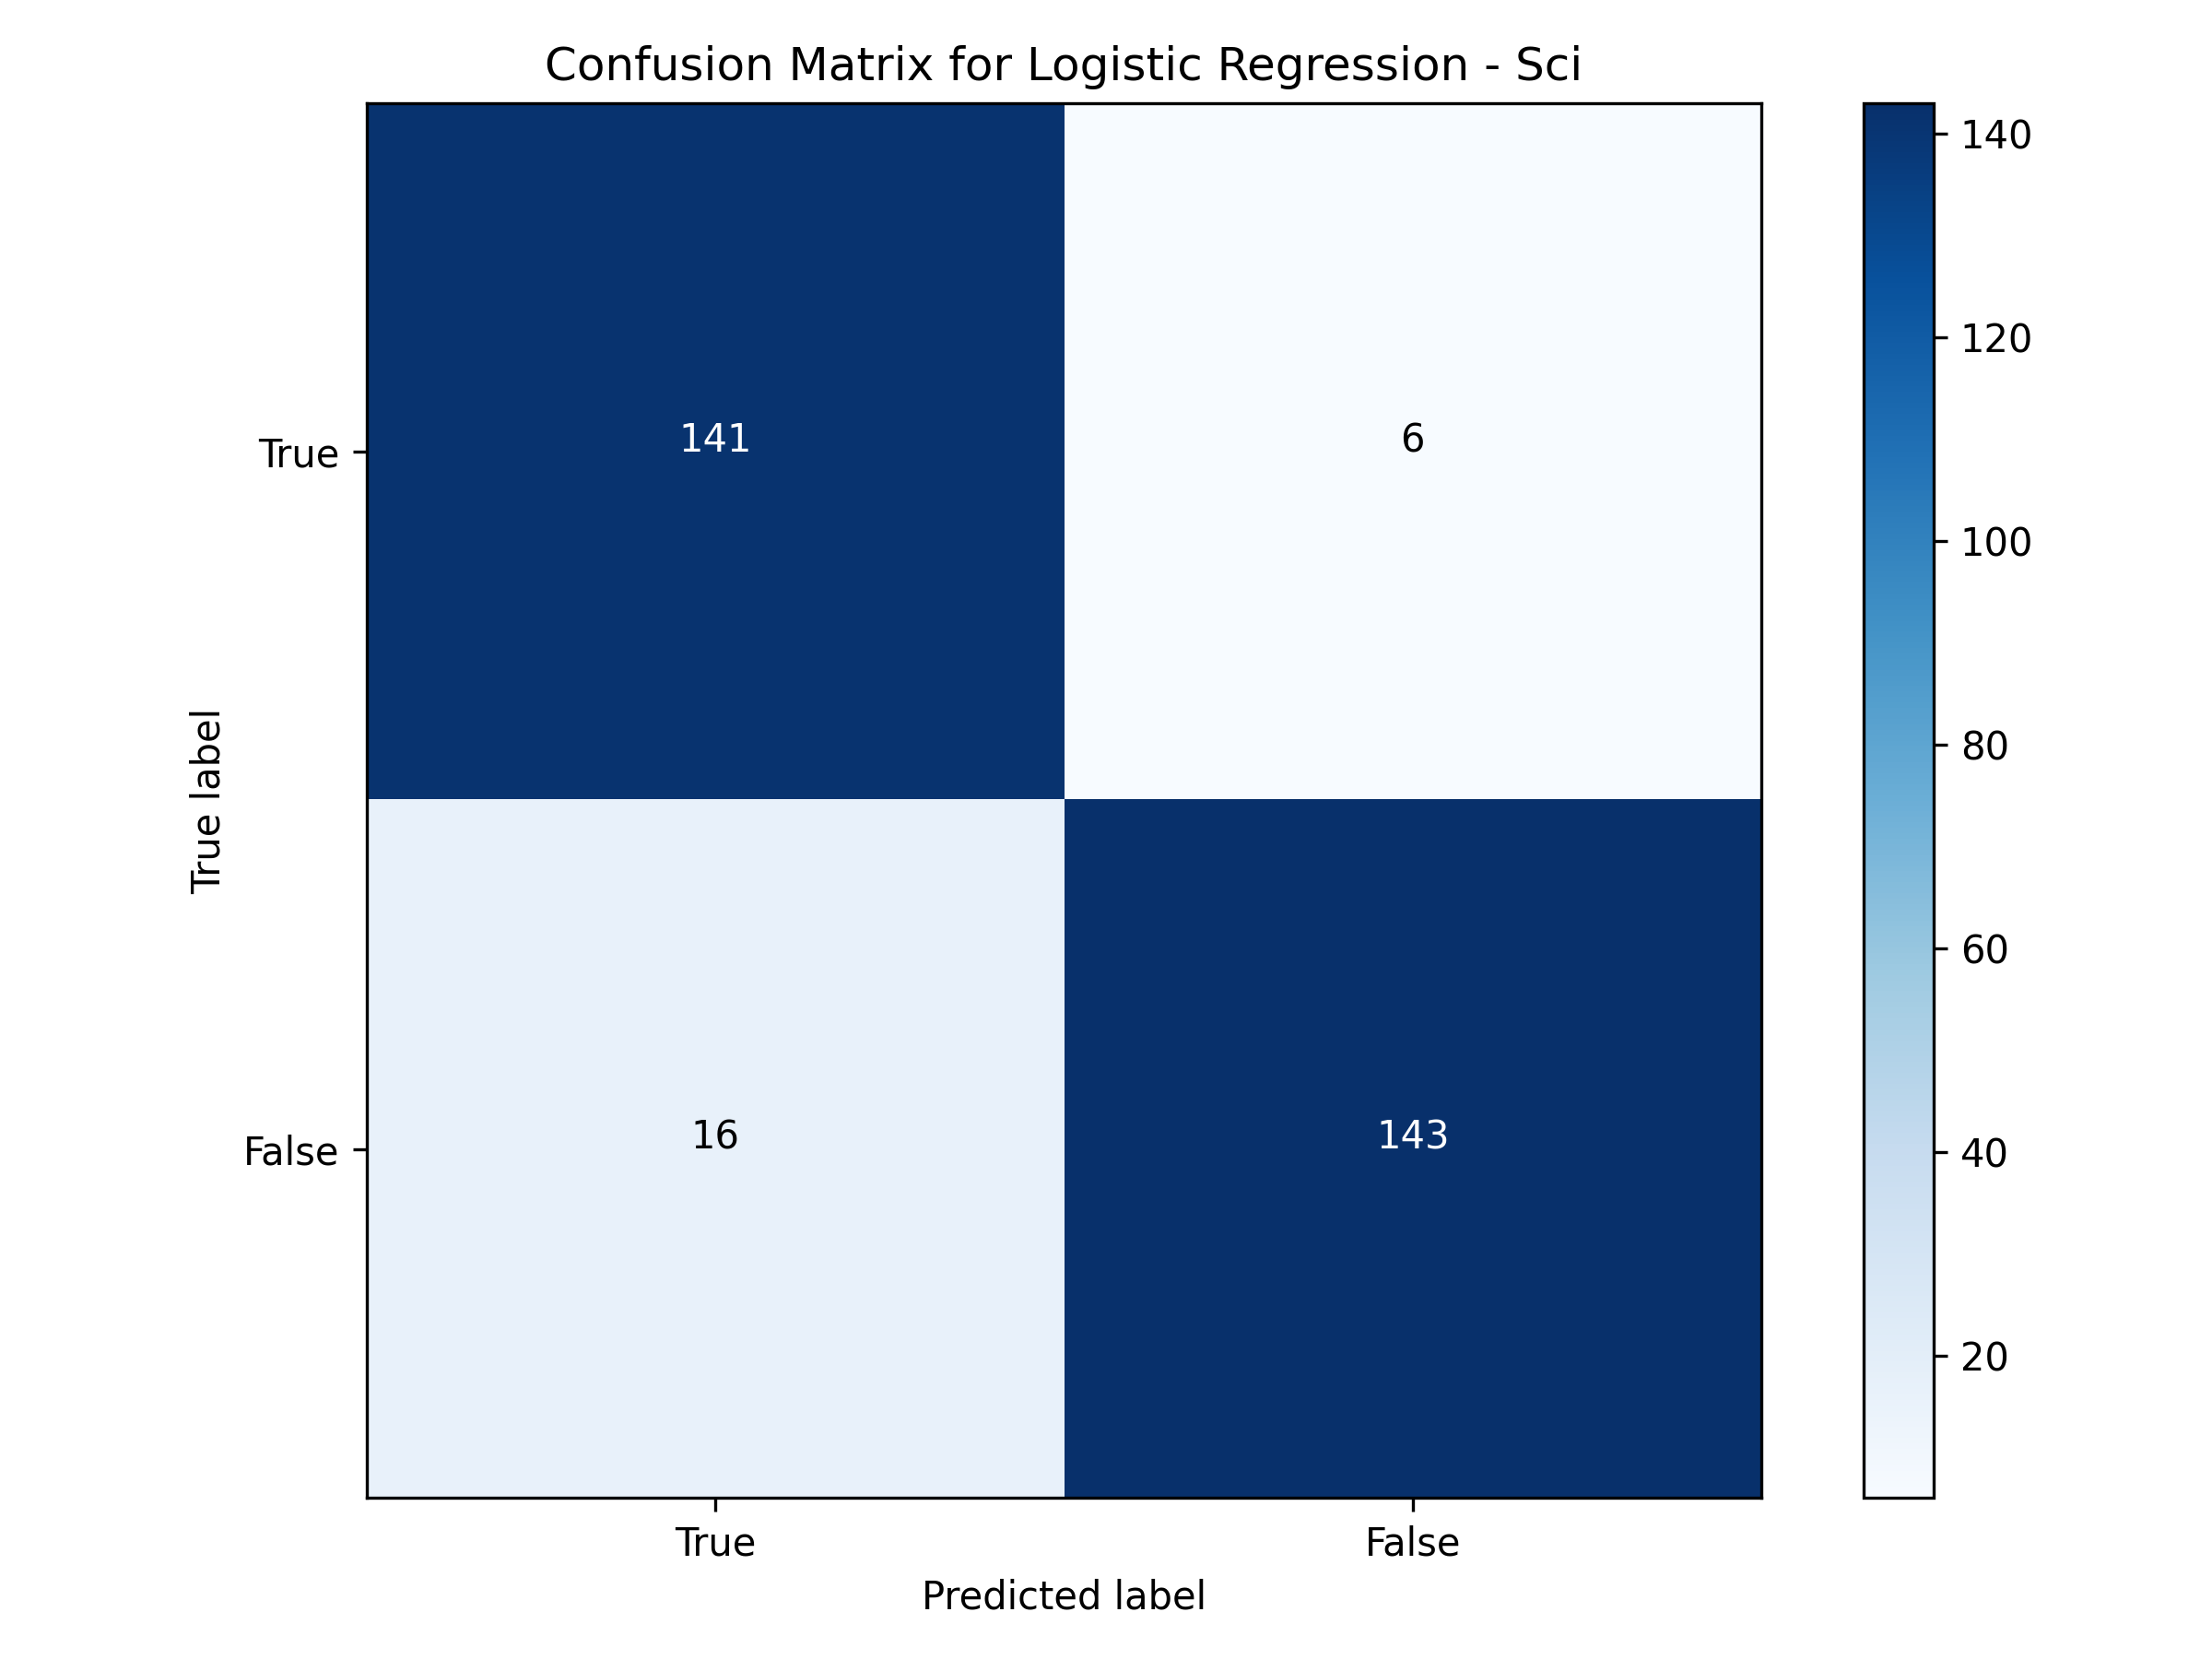
\includegraphics[width=0.49\textwidth]{images/confusion_1.json-Logistic Regression_Sci_confusion_matrix}
    \caption{Matrice de confusion du modèle Logistic Regression pour la classification des tweets scientifiques et non scientifiques.}
    \label{fig:confusion_1.json-logistic-regression_sci_confusion_matrix}
\end{figure}

\subsection{Modèle 2: Affirmation et Référence versus Contexte}\label{subsec:modele-2:-claim-et-ref-vs-contexte}
À présent, nous allons considérer les classes "Affirmation" et "Référence" qui citent une affirmation scientifique d’une part, et la classe "Contexte" qui servent de contexte
D’autre part, toujours afin de réaliser une classification binaire.
Les tweets analysés sont uniquement ceux classés comme scientifiques dans la première tâche.

\subsubsection{Préparation des données}
Le prétraitement textuel a suivi une logique proche de celle adoptée dans la première tâche (minuscules, stop words, lemmatisation), mais sans suppression des mentions et caractères 	spéciaux, afin d’explorer s’ils peuvent porter une valeur contextuelle utile.

La vectorisation a été réalisée à l’aide de TF-IDF, en élargissant la fenêtre aux trigrammes (1 à 3-grammes) afin de mieux capturer les structures linguistiques propres aux énoncés de type affirmation ou citation.

Contrairement à la première tâche, nous n’avons pas appliqué SMOTE Ici, le déséquilibre est partiel dans la distribution des combinaisons de labels (tableau 2,) car la combinaison {1,1} est majoritaire, tandis que la combinaison {0,1} est fortement sous-représentée. La classification est multi-label (un tweet 	peut être à la fois CONTEXT et CLAIM/REF). Nous avons donc  implémenté un rééchantillonnage manuel spécifique au multi-label, en nous basant sur l’identification de toutes les combinaisons de labels possibles et en suréchantillonnant celles qui étaient sous-représentées. 
\begin{figure}[H]
    \centering
    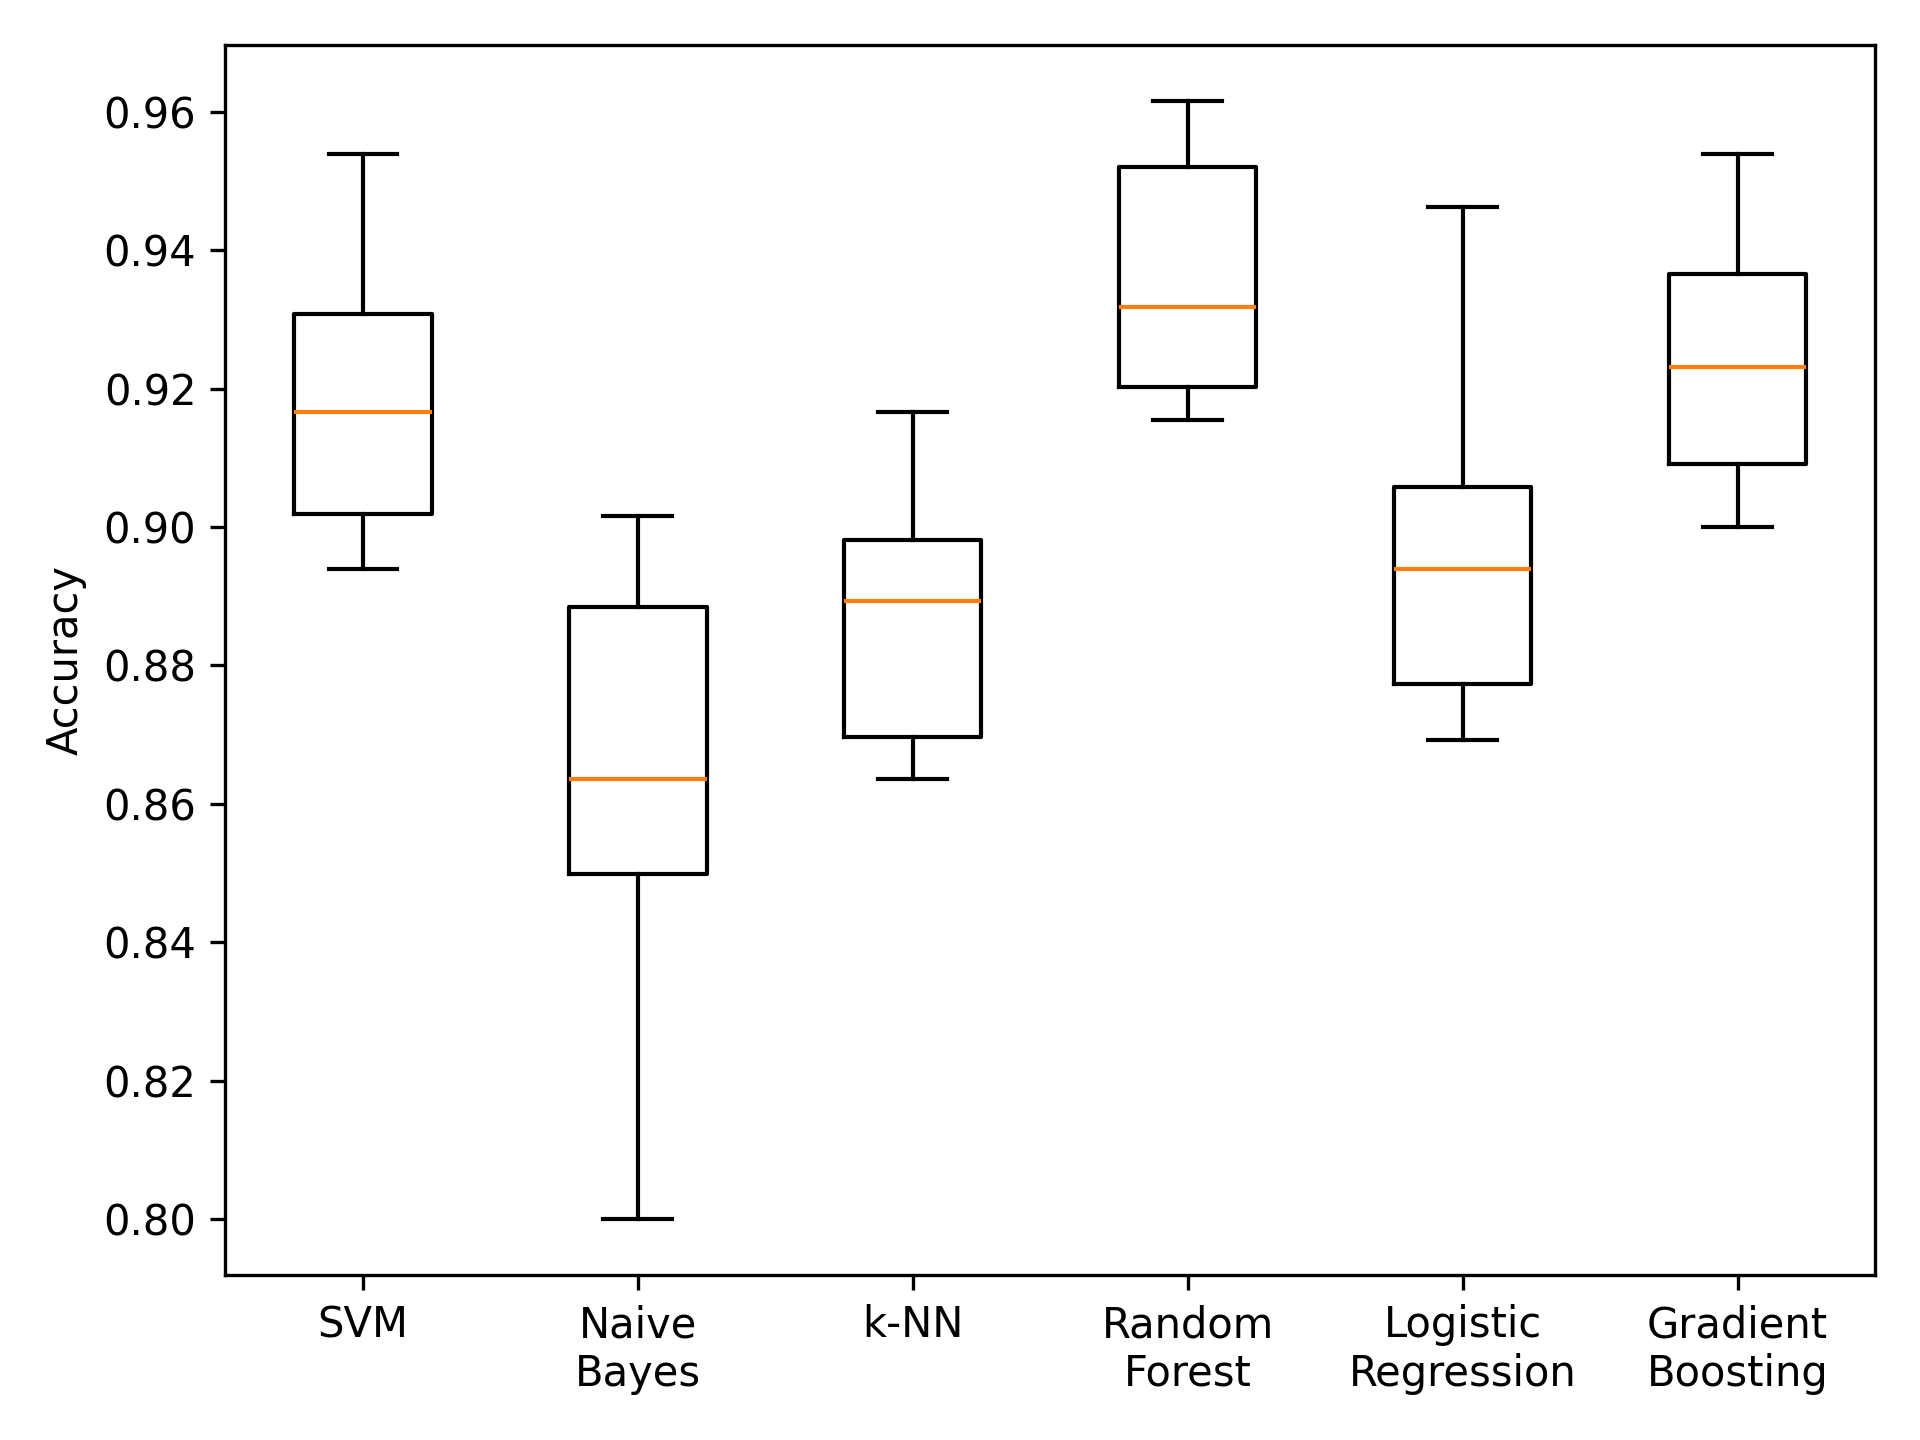
\includegraphics[width=0.75\textwidth]{images/model_comparison_2}
    \caption{Comparaison des modèles pour la classification des tweets claim et ref vs contexte.}
    \label{fig:model_comparison_clmref_context}
\end{figure}

\begin{figure}[h]
    \centering
    \begin{minipage}[b]{0.49\textwidth}
        \centering
        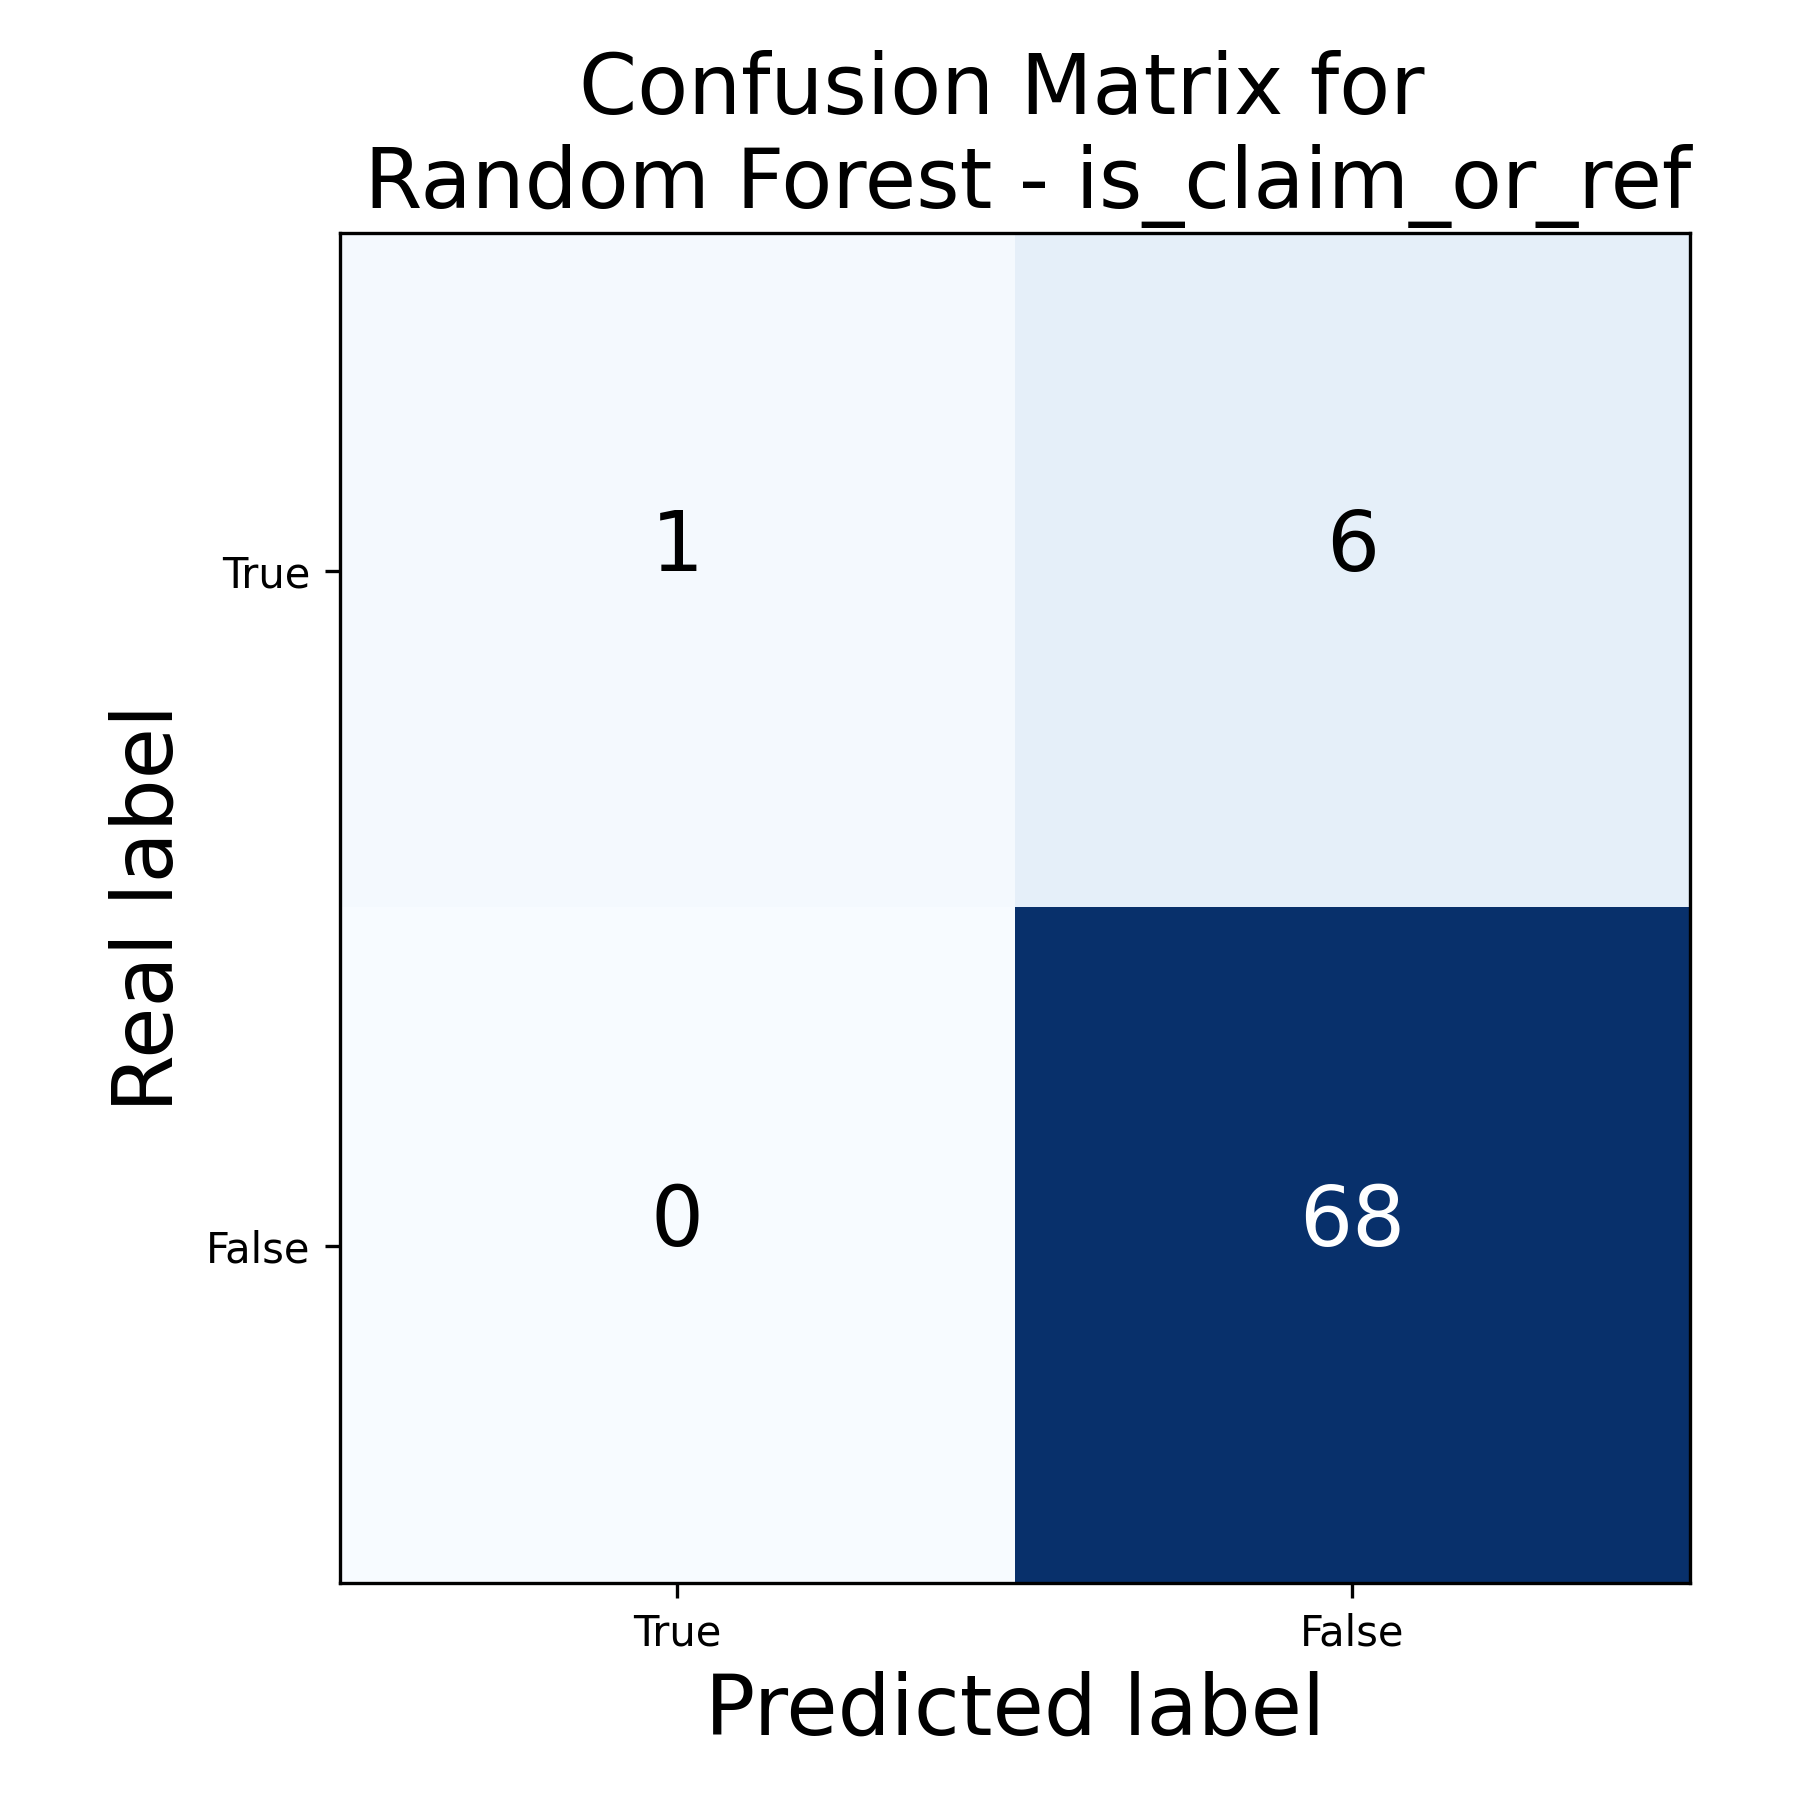
\includegraphics[width=\textwidth]{images/confusion_2.json-Random Forest_is_claim_or_ref_confusion_matrix}
        \label{fig:confusion_2_1}
    \end{minipage}
    \hfill
    \begin{minipage}[b]{0.49\textwidth}
        \centering
        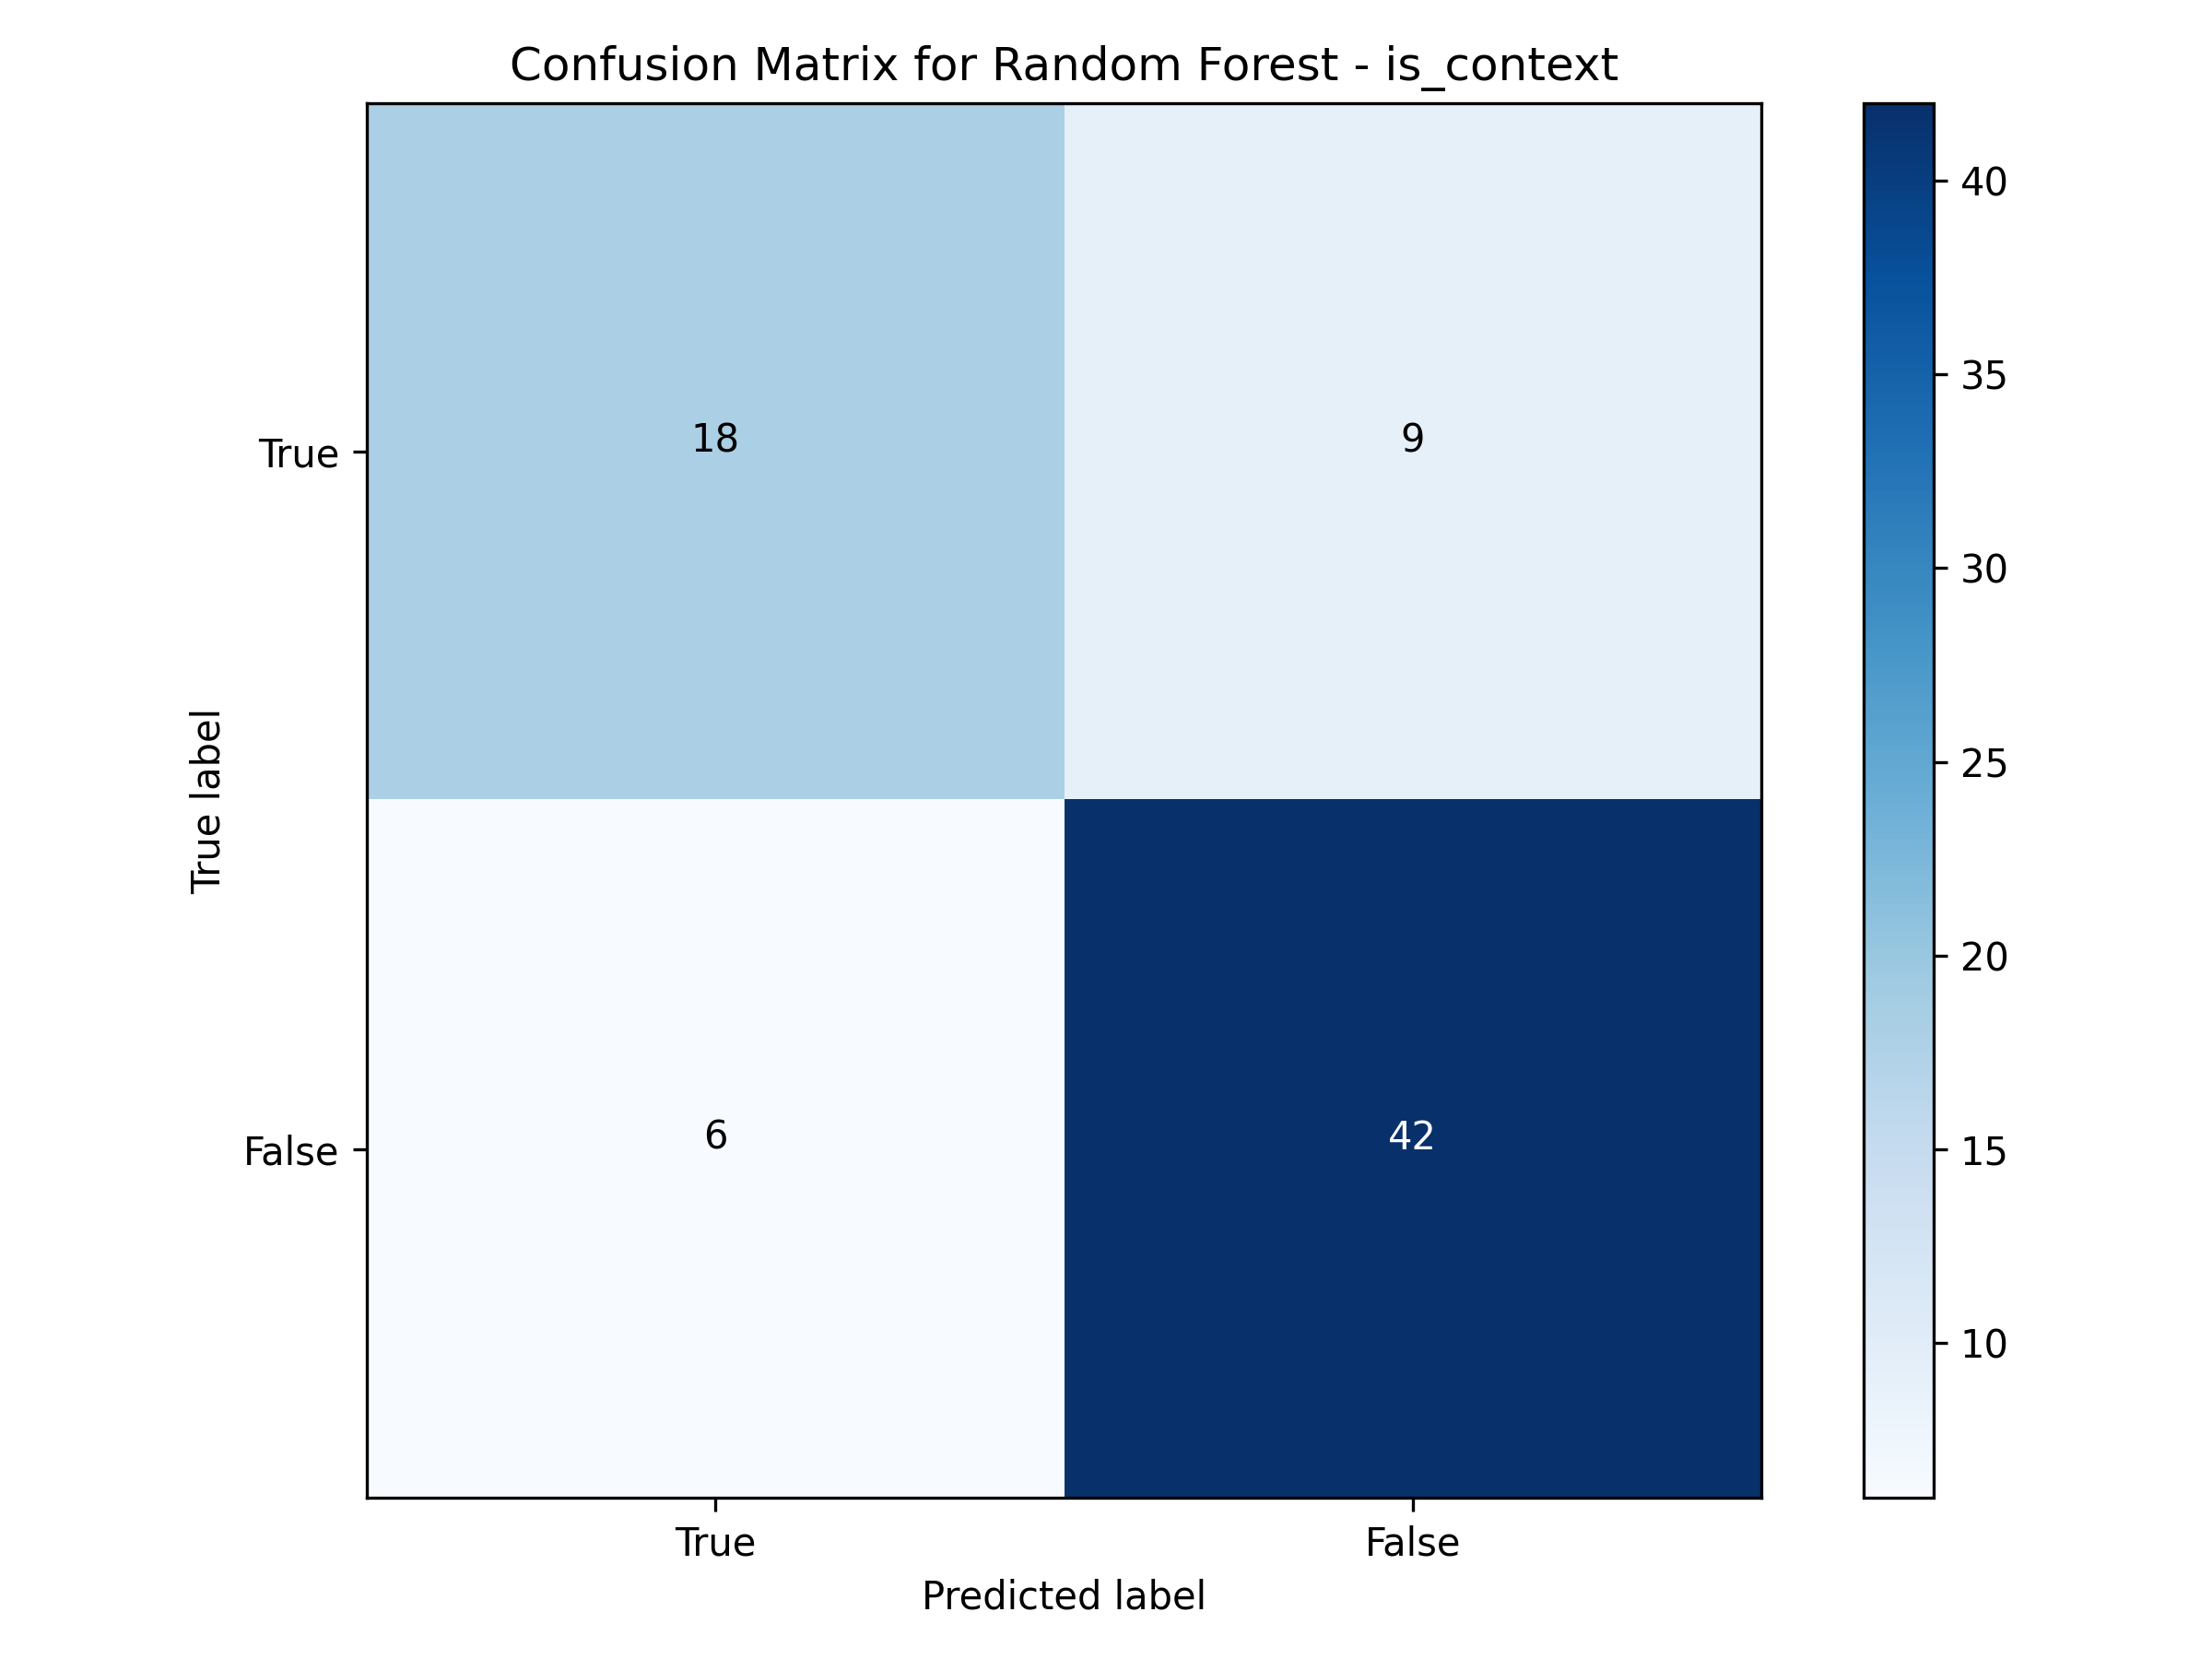
\includegraphics[width=\textwidth]{images/confusion_2.json-Random Forest_is_context_confusion_matrix}
        \label{fig:confusion_2_2}
    \end{minipage}
    \caption{Matrice de confusion du modèle Random Forest pour la classification des tweets claim et ref vs contexte.}
    \label{fig:confusion_2}
\end{figure}

\subsection{Modèle 3: claim vs ref vs contexte}\label{subsec:modele-3:-claim-vs-ref-vs-contexte}
\begin{figure}[H]
    \centering
    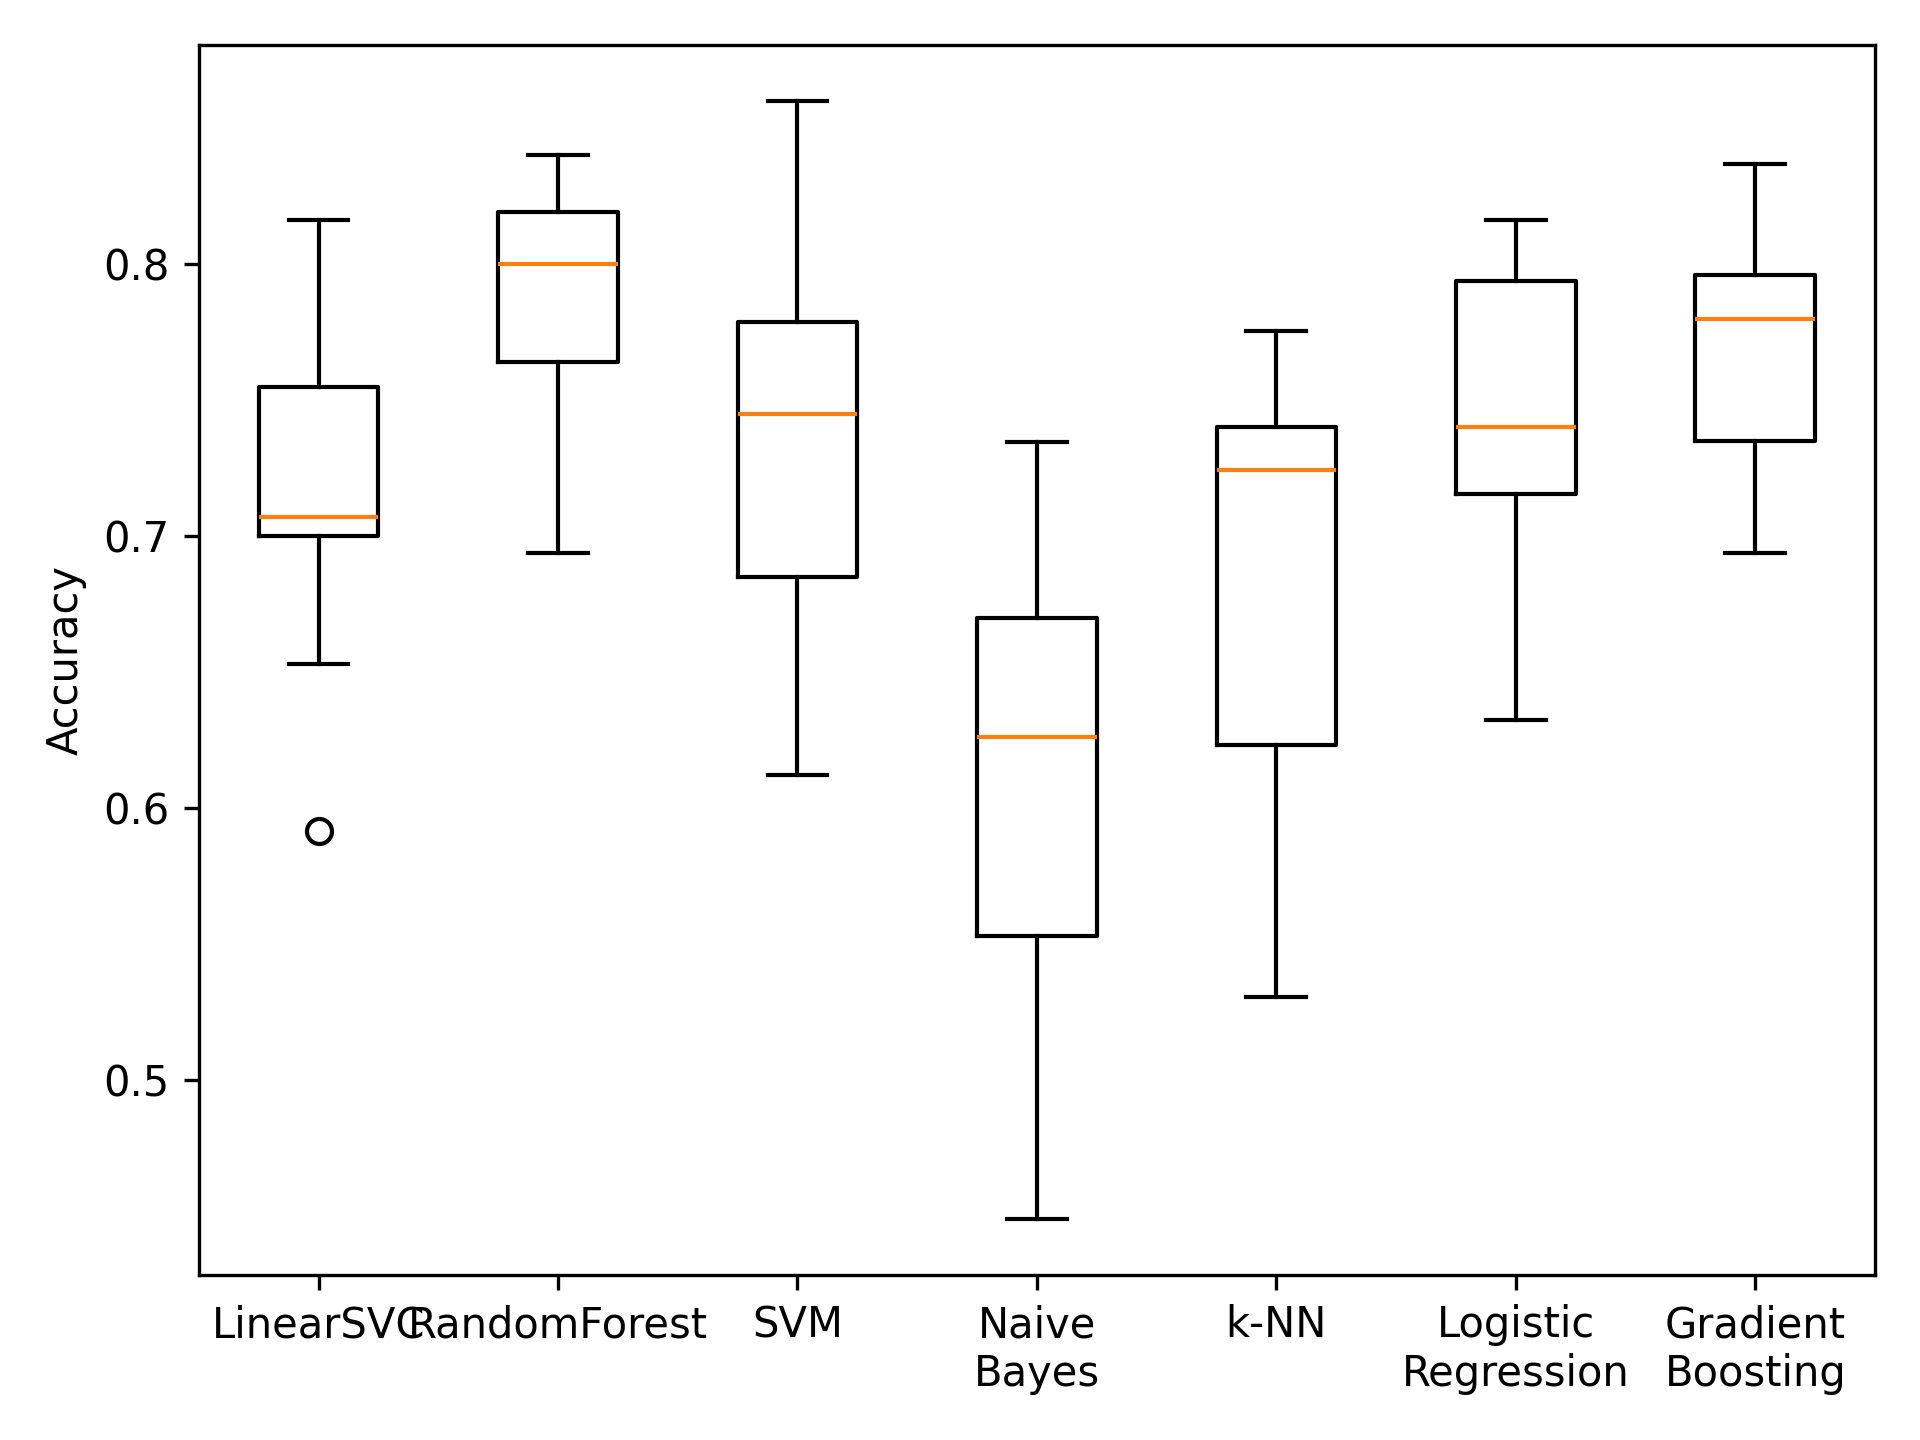
\includegraphics[width=0.75\textwidth]{images/model_comparison_3}
    \caption{Comparaison des modèles pour la classification des tweets claim vs ref vs contexte.}
    \label{fig:model_comparison_clm_ref_context}
\end{figure}

\begin{figure}[h]
    \centering
    \begin{minipage}[b]{0.45\textwidth}
        \centering
        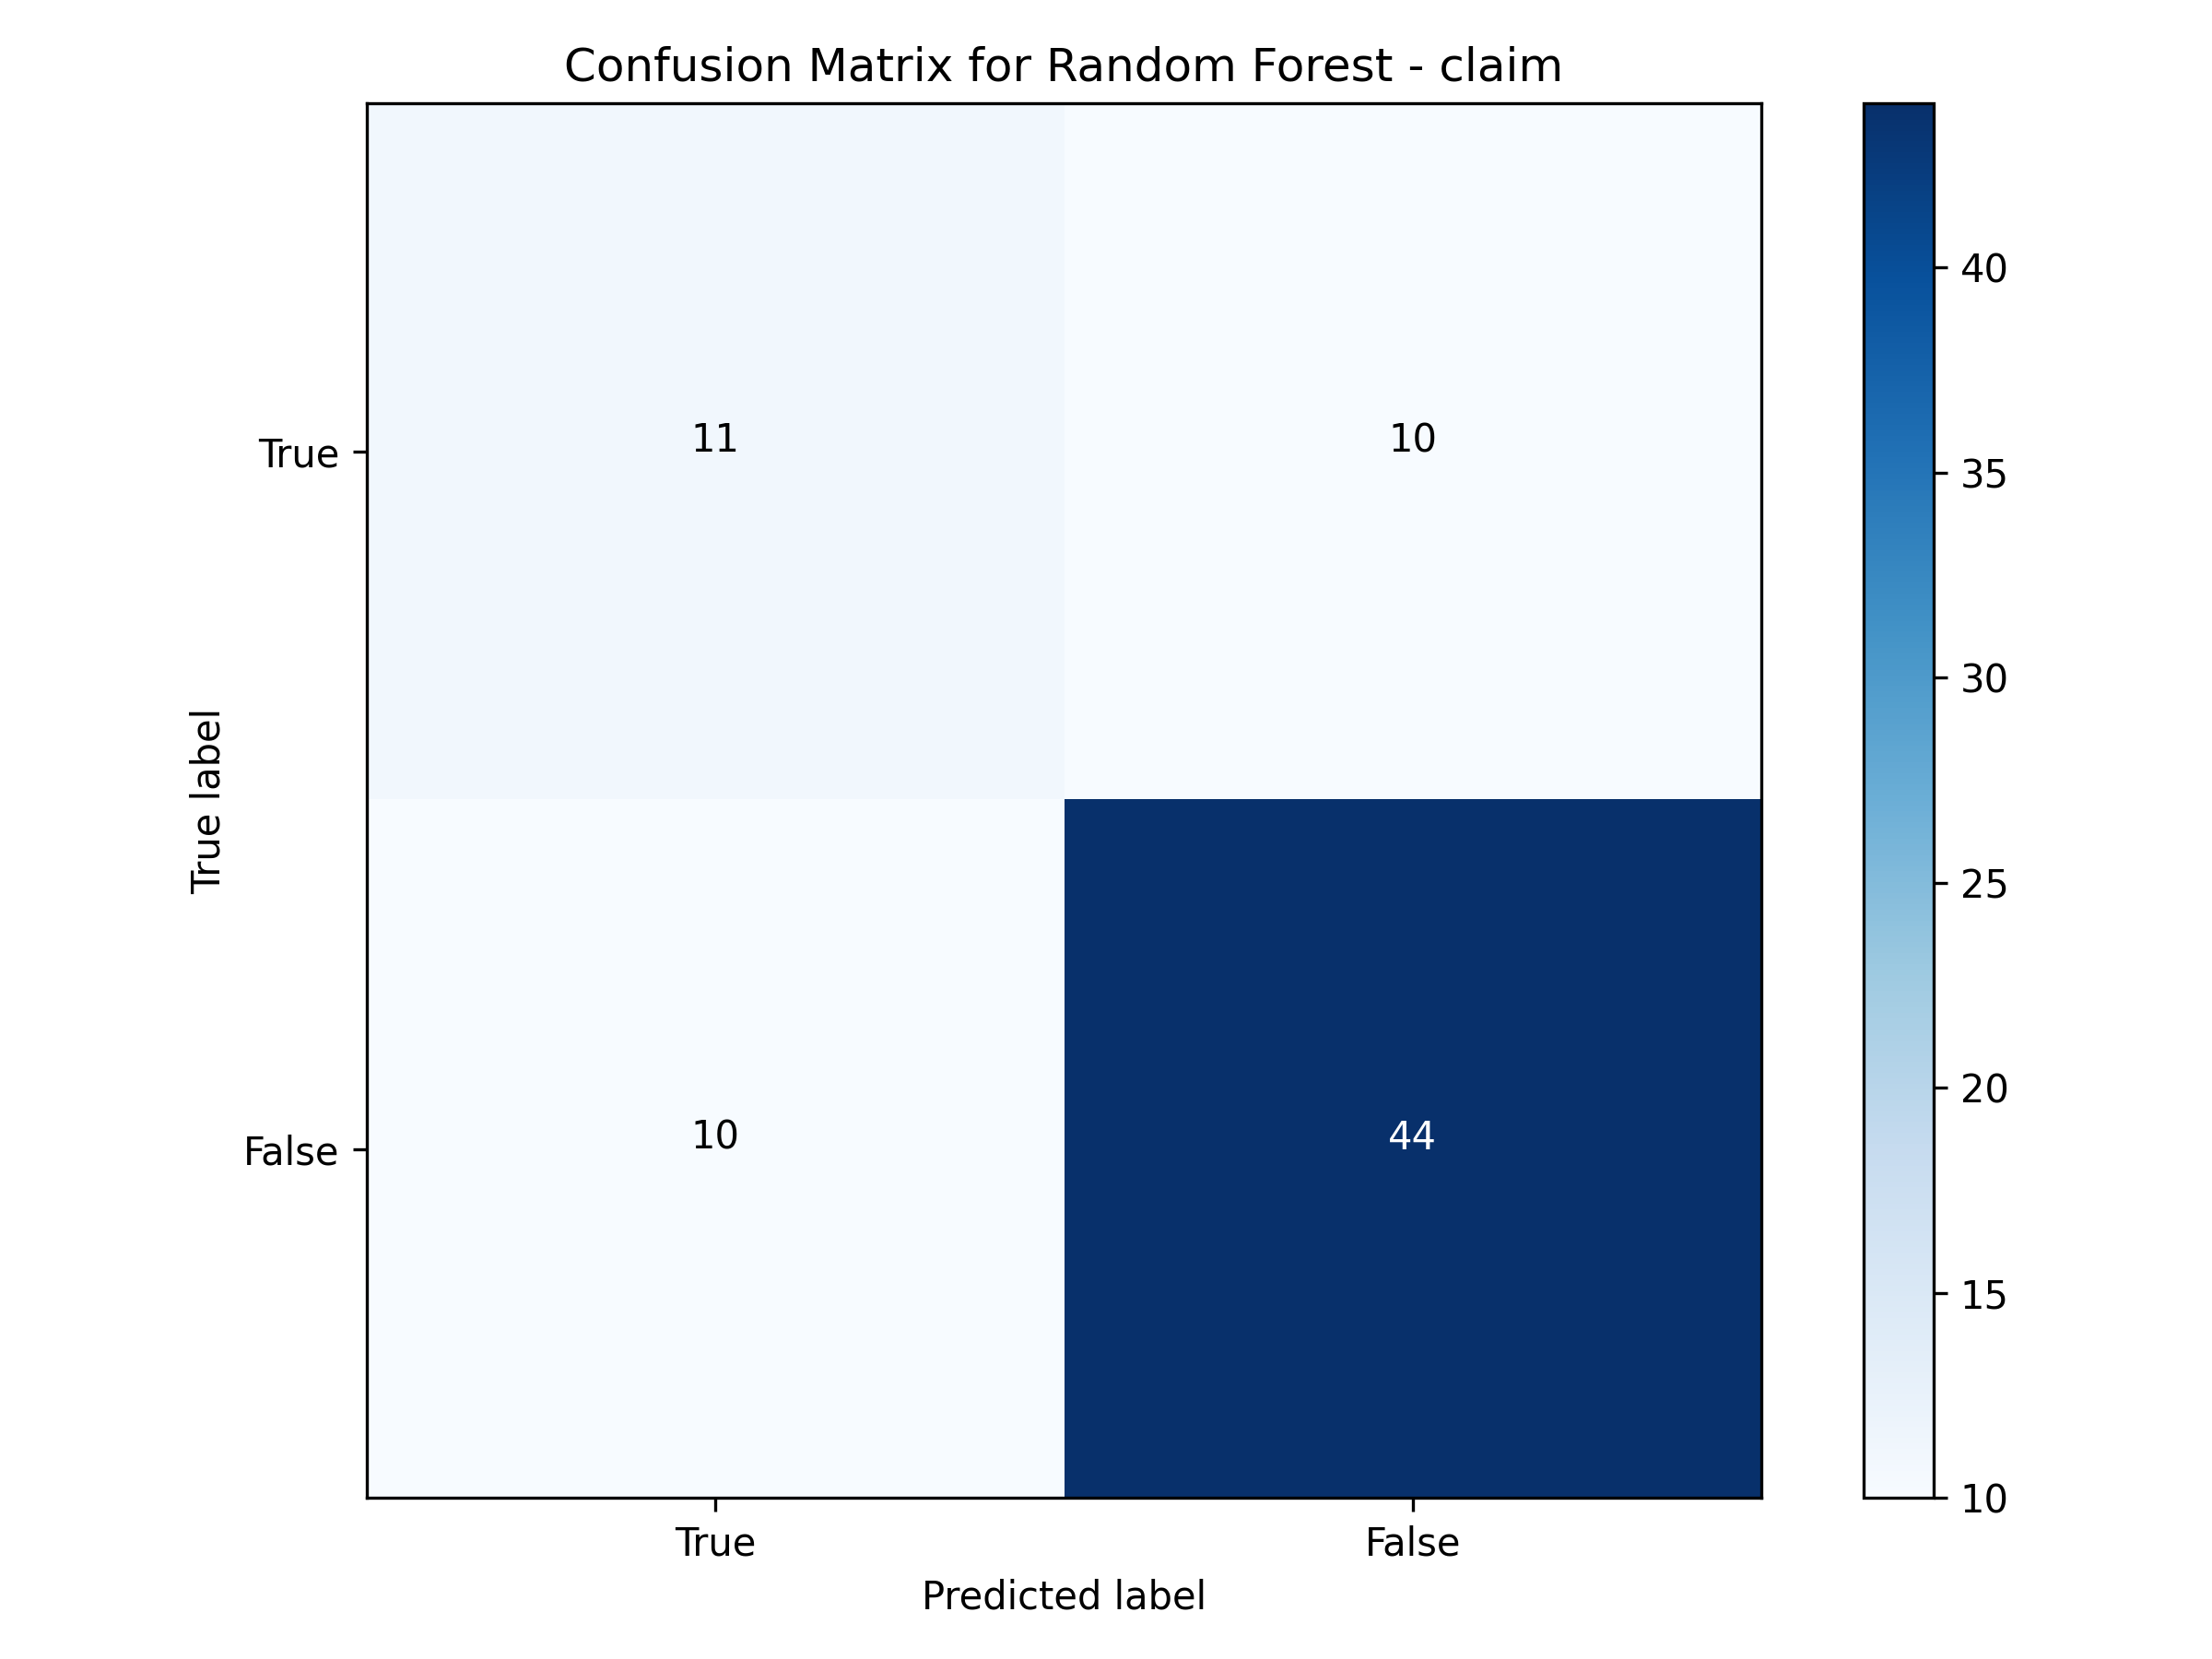
\includegraphics[width=\textwidth]{images/confusion_3.json-Random Forest_claim_confusion_matrix}
        \label{fig:confusion_3_1}
    \end{minipage}
    \hspace{1em}
    \begin{minipage}[b]{0.45\textwidth}
        \centering
        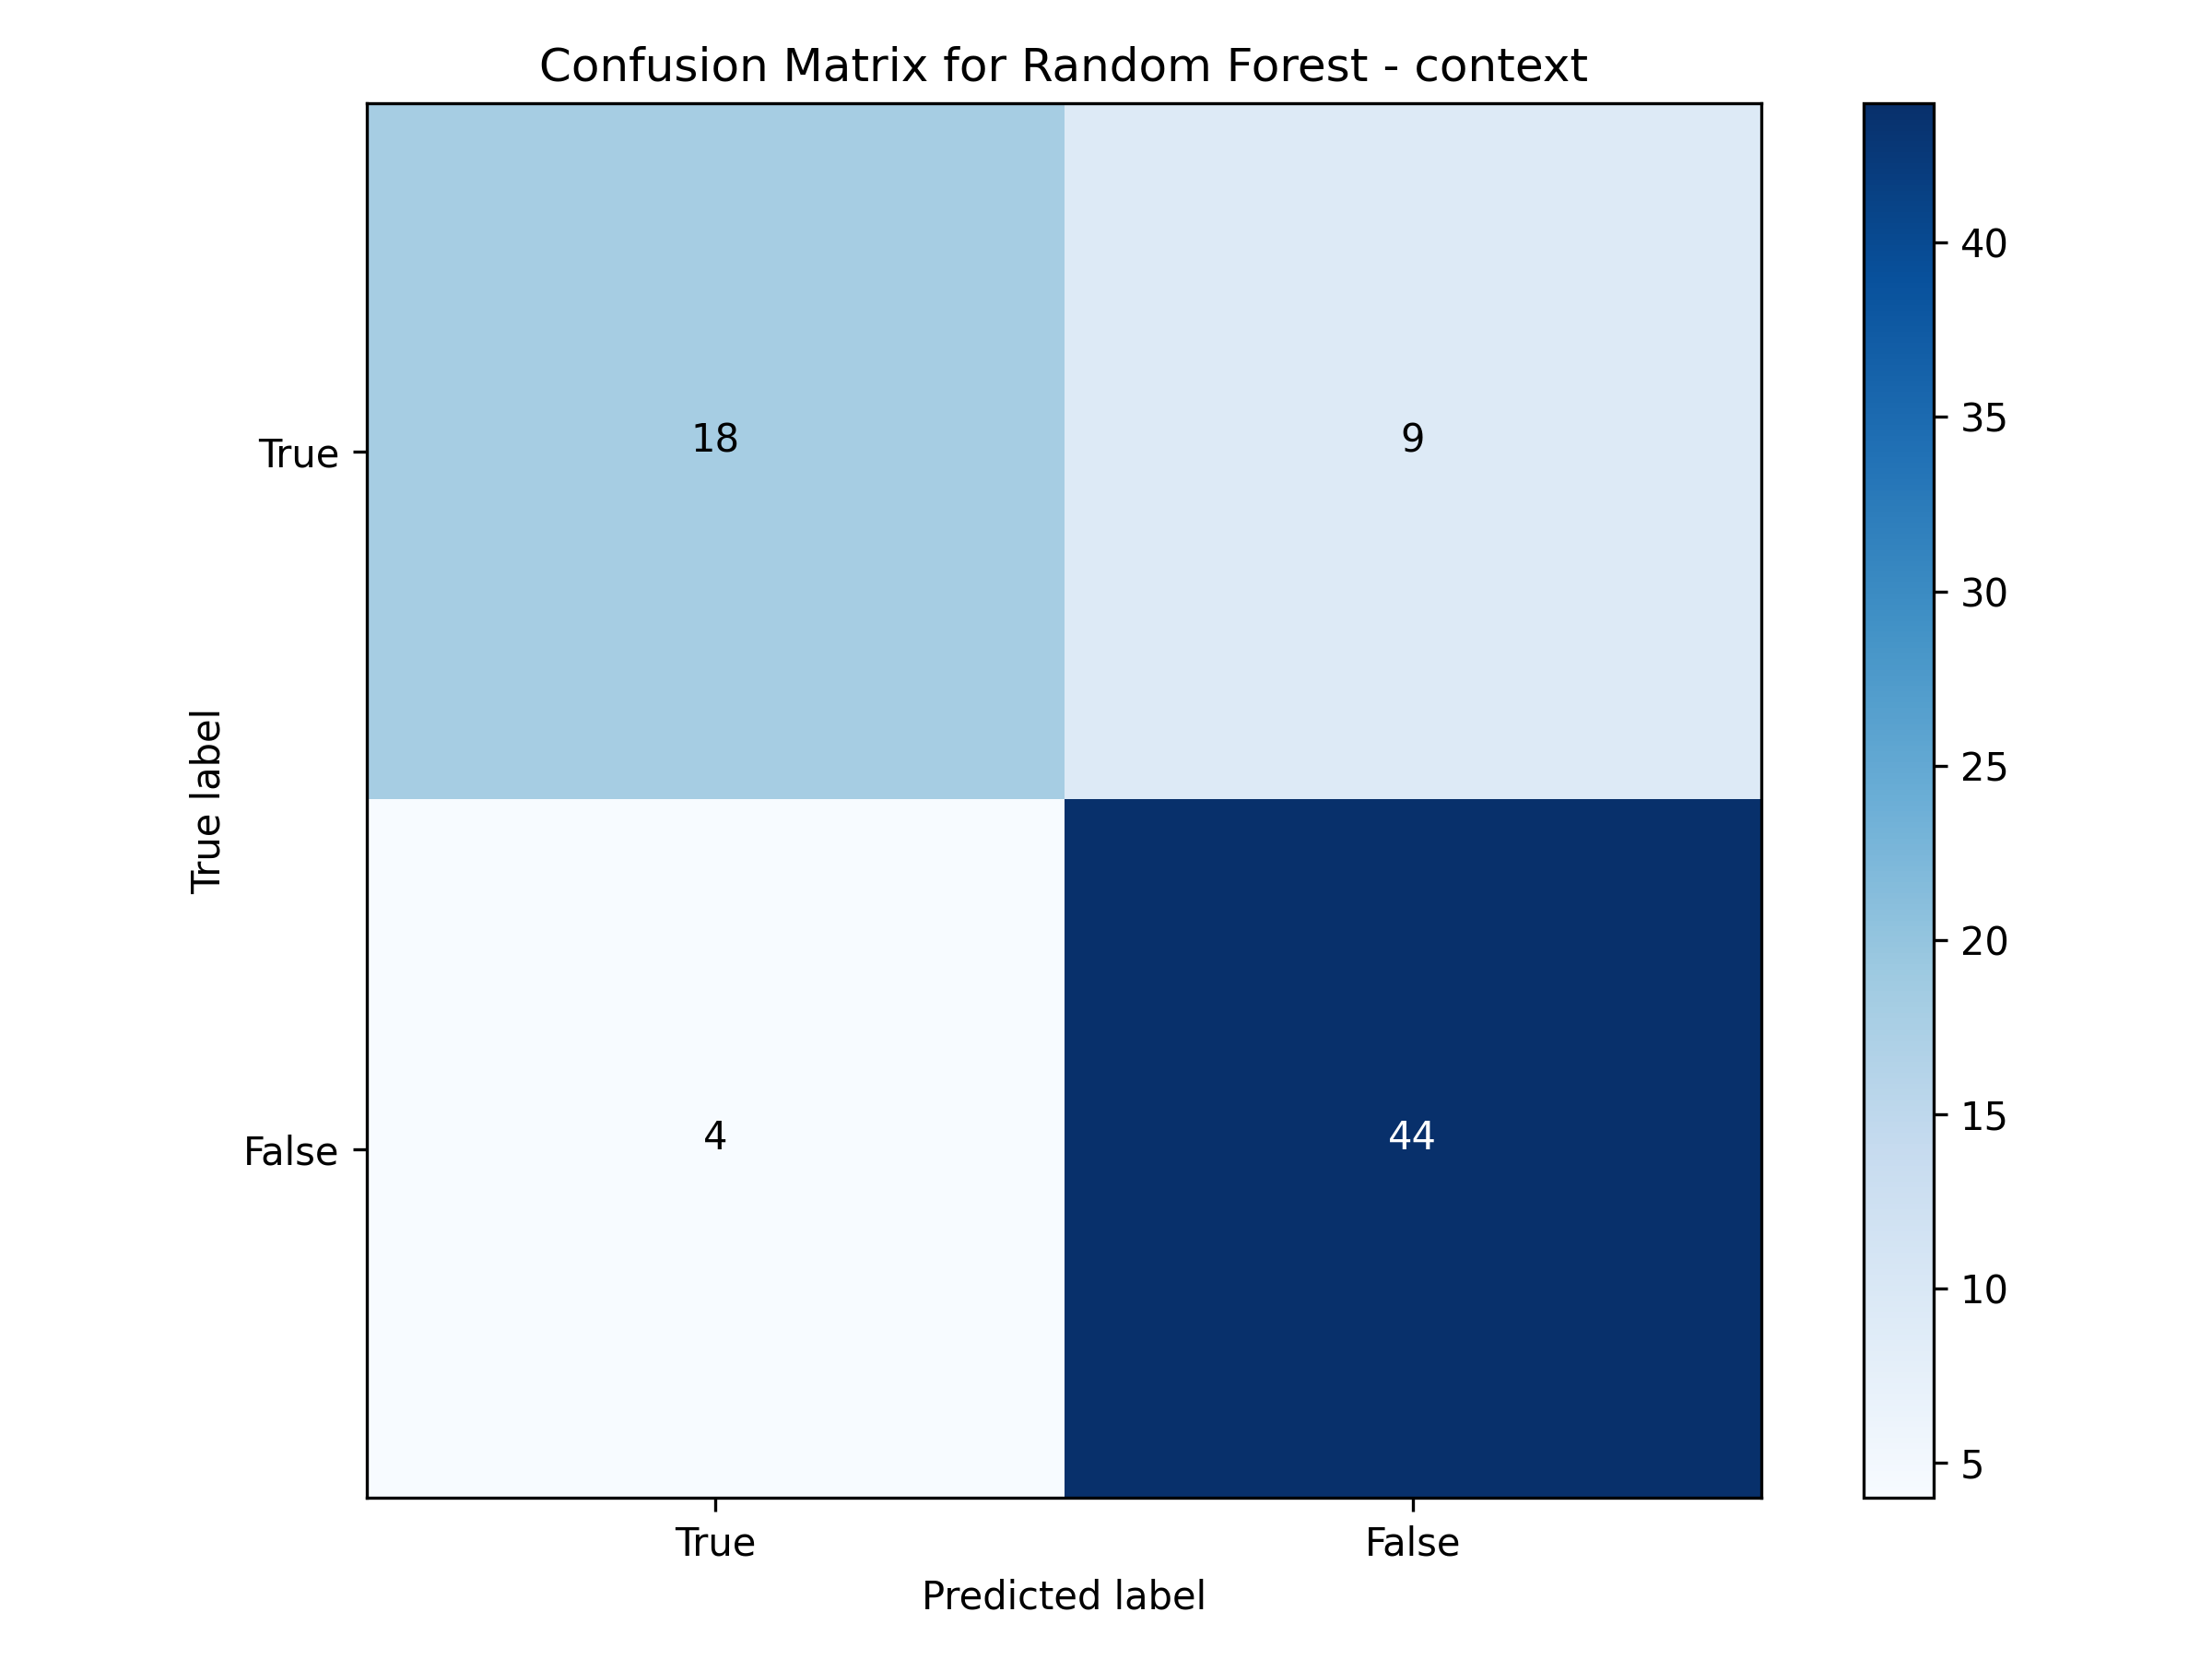
\includegraphics[width=\textwidth]{images/confusion_3.json-Random Forest_context_confusion_matrix}
        \label{fig:confusion_3_2}
    \end{minipage}
    \hspace{1em}
    \begin{minipage}[b]{0.45\textwidth}
        \centering
        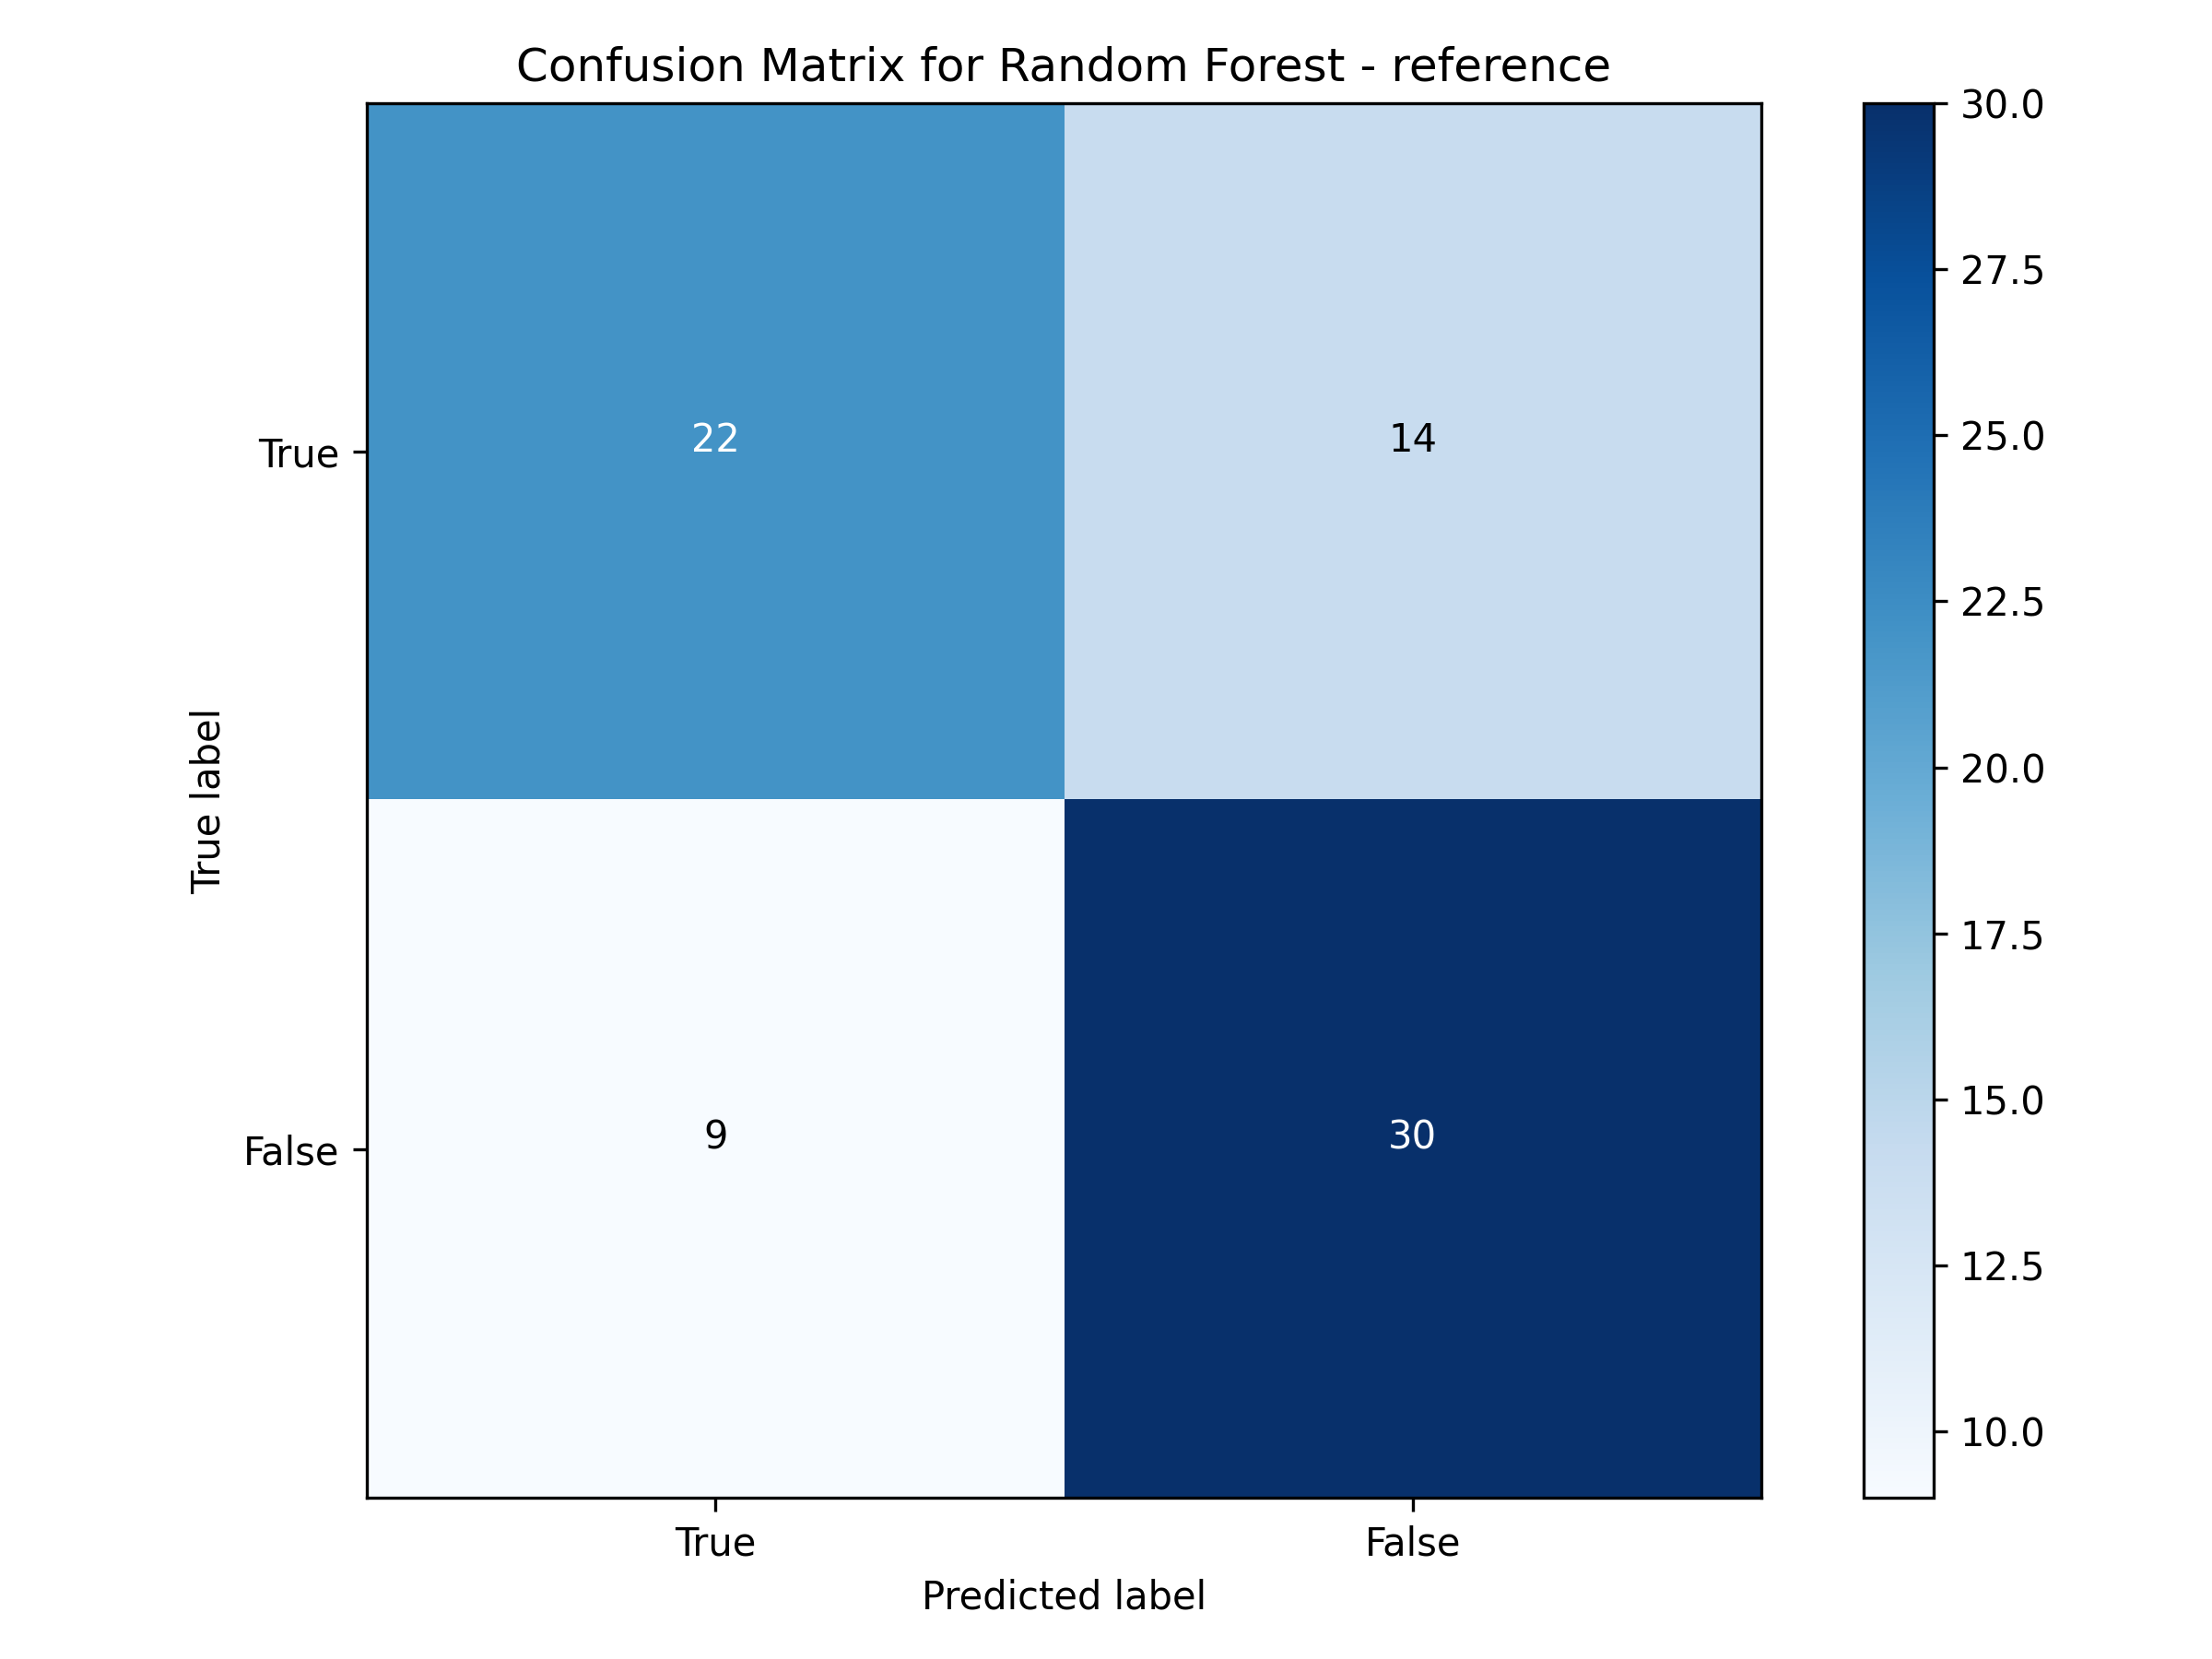
\includegraphics[width=\textwidth]{images/confusion_3.json-Random Forest_reference_confusion_matrix}
        \label{fig:confusion_3_3}
    \end{minipage}
    \caption{Matrice de confusion du modèle Random Forest pour la classification des tweets claim vs ref vs contexte.}
    \label{fig:confusion_3}
\end{figure}